\documentclass[10pt, landscape]{article}
\usepackage[scaled=0.92]{helvet}
\usepackage{calc}
\usepackage{multicol}
\usepackage{ifthen}
\usepackage[a4paper,margin=3mm,landscape]{geometry}
\usepackage{amsmath,amsthm,amsfonts,amssymb}
\usepackage{color,graphicx,overpic}
\usepackage{hyperref}
\usepackage{newtxtext} 
\usepackage{enumitem}
\usepackage{amssymb}
\usepackage[table]{xcolor}
\usepackage{vwcol}
\usepackage{tikz}
\usetikzlibrary{arrows.meta}
\usetikzlibrary{calc}
\usepackage{mathtools}
\usepackage{nicematrix}
%For pictures / figures
\usepackage{color,graphicx,overpic}
\graphicspath{ {./images/} }
% for relations
\usepackage{cancel}
\usepackage{ mathrsfs }
\graphicspath{ {./images/} }
\setlist{nosep}

\pdfinfo{
  /Title (CG1111A-Quiz2.pdf)
  /Creator (TeX)
  /Producer (pdfTeX 1.40.0)
  /Author (Seamus)
  /Subject (Example)
  /Keywords (pdflatex, latex,pdftex,tex)}

% Turn off header and footer
\pagestyle{empty}

\newenvironment{tightcenter}{%
  \setlength\topsep{0pt}
  \setlength\parskip{0pt}
  \begin{center}
}{%
  \end{center}
}

% redefine section commands to use less space
\makeatletter
\renewcommand{\section}{\@startsection{section}{1}{0mm}%
                                {-1ex plus -.5ex minus -.2ex}%
                                {0.5ex plus .2ex}%x
                                {\normalfont\large\bfseries}}
\renewcommand{\subsection}{\@startsection{subsection}{2}{0mm}%
                                {-1explus -.5ex minus -.2ex}%
                                {0.5ex plus .2ex}%
                                {\normalfont\normalsize\bfseries}}
\renewcommand{\subsubsection}{\@startsection{subsubsection}{3}{0mm}%
                                {-1ex plus -.5ex minus -.2ex}%
                                {1ex plus .2ex}%
                                {\normalfont\small\bfseries}}%
\renewcommand{\familydefault}{\sfdefault}
\renewcommand\rmdefault{\sfdefault}
% makes nested numbering (e.g. 1.1.1, 1.1.2, etc)
\renewcommand{\labelenumii}{\theenumii}
\renewcommand{\theenumii}{\theenumi.\arabic{enumii}.}
\renewcommand\labelitemii{•}
%  for logical not operator
\renewcommand{\lnot}{\mathord{\sim}}
\renewcommand{\bf}[1]{\textbf{#1}}
\newcommand{\abs}[1]{\vert #1 \vert}
\newcommand{\Mod}[1]{\ \mathrm{mod}\ #1}

\makeatother
\definecolor{myblue}{cmyk}{1,.72,0,.38}
\everymath\expandafter{\the\everymath \color{myblue}}
% Define BibTeX command
\def\BibTeX{{\rm B\kern-.05em{\sc i\kern-.025em b}\kern-.08em
    T\kern-.1667em\lower.7ex\hbox{E}\kern-.125emX}}
\let\iff\leftrightarrow
\let\Iff\Leftrightarrow
\let\then\rightarrow
\let\Then\Rightarrow

% Don't print section numbers
\setcounter{secnumdepth}{0}

\setlength{\parindent}{0pt}
\setlength{\parskip}{0pt plus 0.5ex}
%% this changes all items (enumerate and itemize)
\setlength{\leftmargini}{0.5cm}
\setlength{\leftmarginii}{0.5cm}
\setlist[itemize,1]{leftmargin=2mm,labelindent=1mm,labelsep=1mm}
\setlist[itemize,2]{leftmargin=4mm,labelindent=1mm,labelsep=1mm}

%My Environments
\newtheorem{example}[section]{Example}
% -----------------------------------------------------------------------

\begin{document}
\raggedright
\footnotesize
\begin{multicols}{4}


% multicol parameters
% These lengths are set only within the two main columns
\setlength{\columnseprule}{0.25pt}
\setlength{\premulticols}{1pt}
\setlength{\postmulticols}{1pt}
\setlength{\multicolsep}{1pt}
\setlength{\columnsep}{2pt}

\begin{center}
    \fbox{%
        \parbox{0.8\linewidth}{\centering \textcolor{black}{
            {\Large\textbf{CG1111A Quiz 2}}
            \\ \normalsize{AY24/25 sem 1}}
            \\ {\footnotesize \textcolor{myblue}{github.com/mendax1234}} 
        }%
    }
\end{center}

\section{01. (Studio 7) Transformers and Diode}
\subsection{Principles of Transformers}
\begin{enumerate}
    \item (\textbf{Magnetic Flux}) DC source $\rightarrow$ \textbf{Constant} magnetic flux. AC source $\rightarrow$ \textbf{varying} magnetic flux.
    \item (\textbf{Faraday's Law}) $e=N\frac{d\phi}{dt}$. It means that the change in magnetic flux will cause \textbf{induced electromotive force (EMF)}.
    \item (\textbf{Voltage Ratio}) For an \textbf{ideal} transformer, we have $\frac{V_1}{V_2}=\frac{N_1}{N_2}$\\
    \centerline{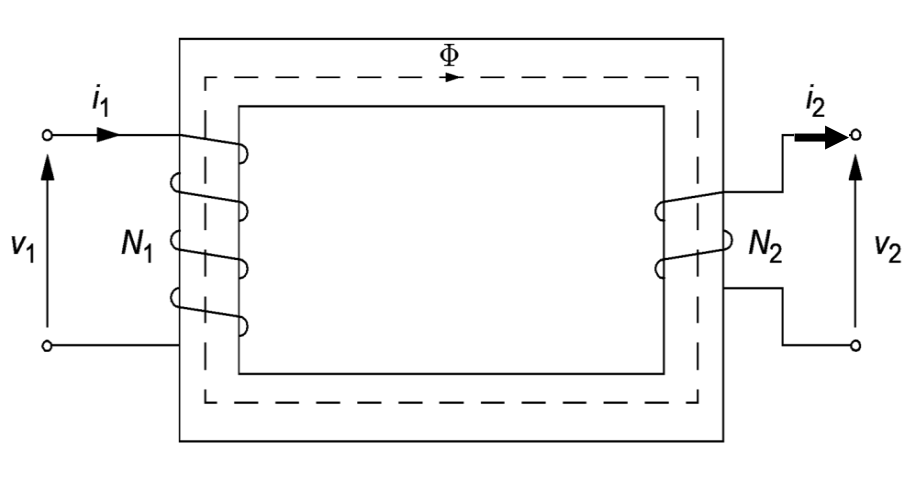
\includegraphics[width=0.5\linewidth]{images/voltage-ratio.png}}
    \item (\textbf{Current Ratio}) For an \textbf{ideal} transformer, we have $i_1N_1=i_2N_2$ or $\frac{i_1}{i_2}=\frac{N_2}{N_1}$
    \item (\textbf{Power}) An \textbf{ideal} transformer has \textbf{no real/reactive power loss}. That's because $S_1=V_1I_1^*=aV_2(\frac{I_2}{a})^*=V_2I_2^*=S_2$, where $*$ means \textit{conjugate}. 
    \item (\textbf{Tips})
    \begin{itemize}
        \item When doing the \textbf{voltage ratio} calculation, just \textbf{ignore the phasor angle} of the voltage (both primary and secondary) and use the \textbf{magnitude} to calculate because in transformer, we care more about the magnitude.
        \item If the secondary side of the transformer is a series RLC load (or anything else), it will be safe to draw a phasor diagram to calculate its voltage, get the value in \textbf{magnitude} also and don't care about the angle. \\
        \centerline{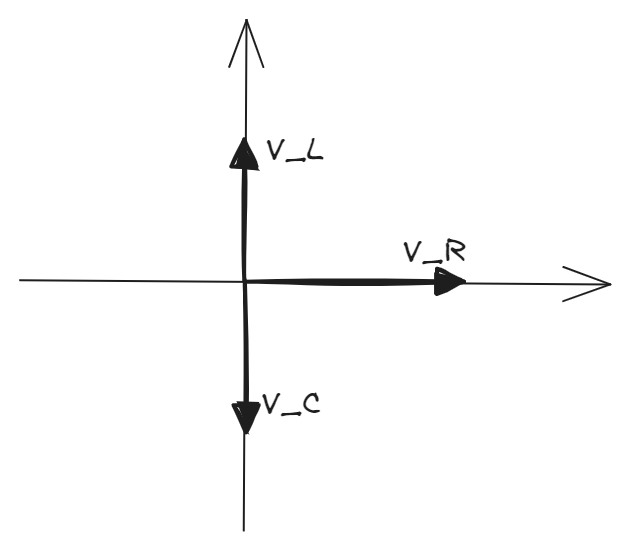
\includegraphics[width=0.5\linewidth]{images/series-rlc.png}}
        (The current also has phase angle, for the current flowing through a capacitor, its phase angle is $-90^\circ$. For the current flowing through a inductor, its phase angle is $90^\circ$)
    \end{itemize}
\end{enumerate}

\subsection{Diode and Diode Bridge Rectifiers}
\begin{enumerate}
    \item (\textbf{Characteristics}) Diode is a \textbf{polarized} device that allows current to flow only in one direction. The positive side $+$ is called the \textbf{anode} and the negative side $-$ is called the \textbf{cathode}.
    \item (\textbf{Forward Biased})
    \begin{itemize}
        \item Diode is \textbf{forward biased} when a \textbf{positive} voltage is applied across the diode. i.e. the anode is at a \textbf{higher} voltage compared to the cathode.
        \item Only when the applied voltage exceeds a \textbf{threshold}, the diode starts to conduct current.
        \item Current grows \textbf{exponentially} with increment voltage beyond this threshold.
    \end{itemize}
    \centerline{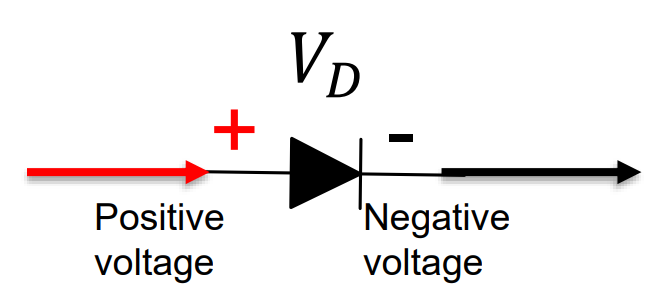
\includegraphics[width=0.5\linewidth]{images/forward-biased-diode.png}}
    \item (\textbf{Reverse Biased})
    \begin{itemize}
        \item Similarly, in this case, a \textbf{negative} voltage is applied to the diode.
        \item \textbf{Negligible current} flows through the diode in this state.
        \item When the reverse-biased voltage is beyond a limit, the diode \textbf{breaks down}. The limit is called \textbf{breakdown limit}.
    \end{itemize}
    \centerline{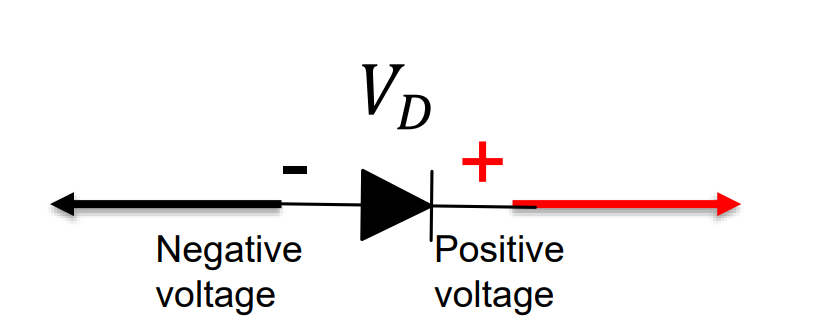
\includegraphics[width=0.6\linewidth]{images/reversed-biased-diode.png}}
    Below is the Diode I-V Characteristics \\
    \centerline{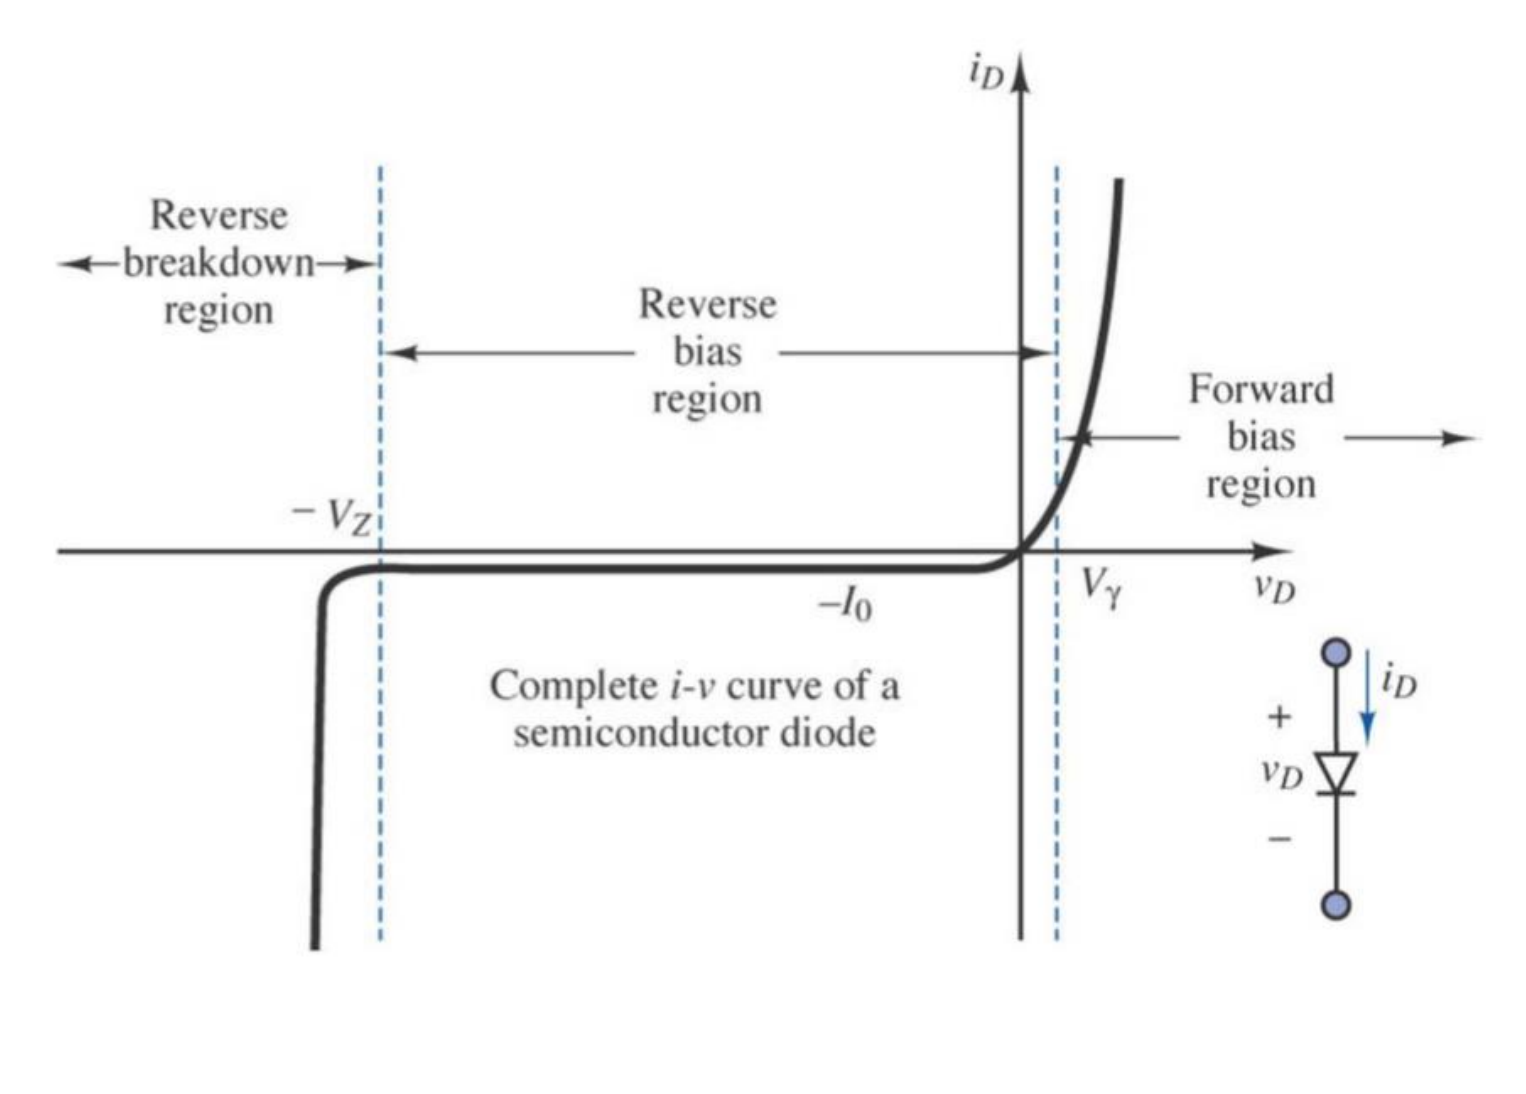
\includegraphics[width=0.8\linewidth]{images/diode-IV-characteristic.png}}
    \item (\textbf{Rectifier}) A \textbf{rectifier} is a circuit which converts alternating current (AC) to direct current (DC).
    \item (\textbf{Diode Bridge Rectifier}) The following graph summarises the working principle of diode bridge rectifier using the characteristics above. \\
    \centerline{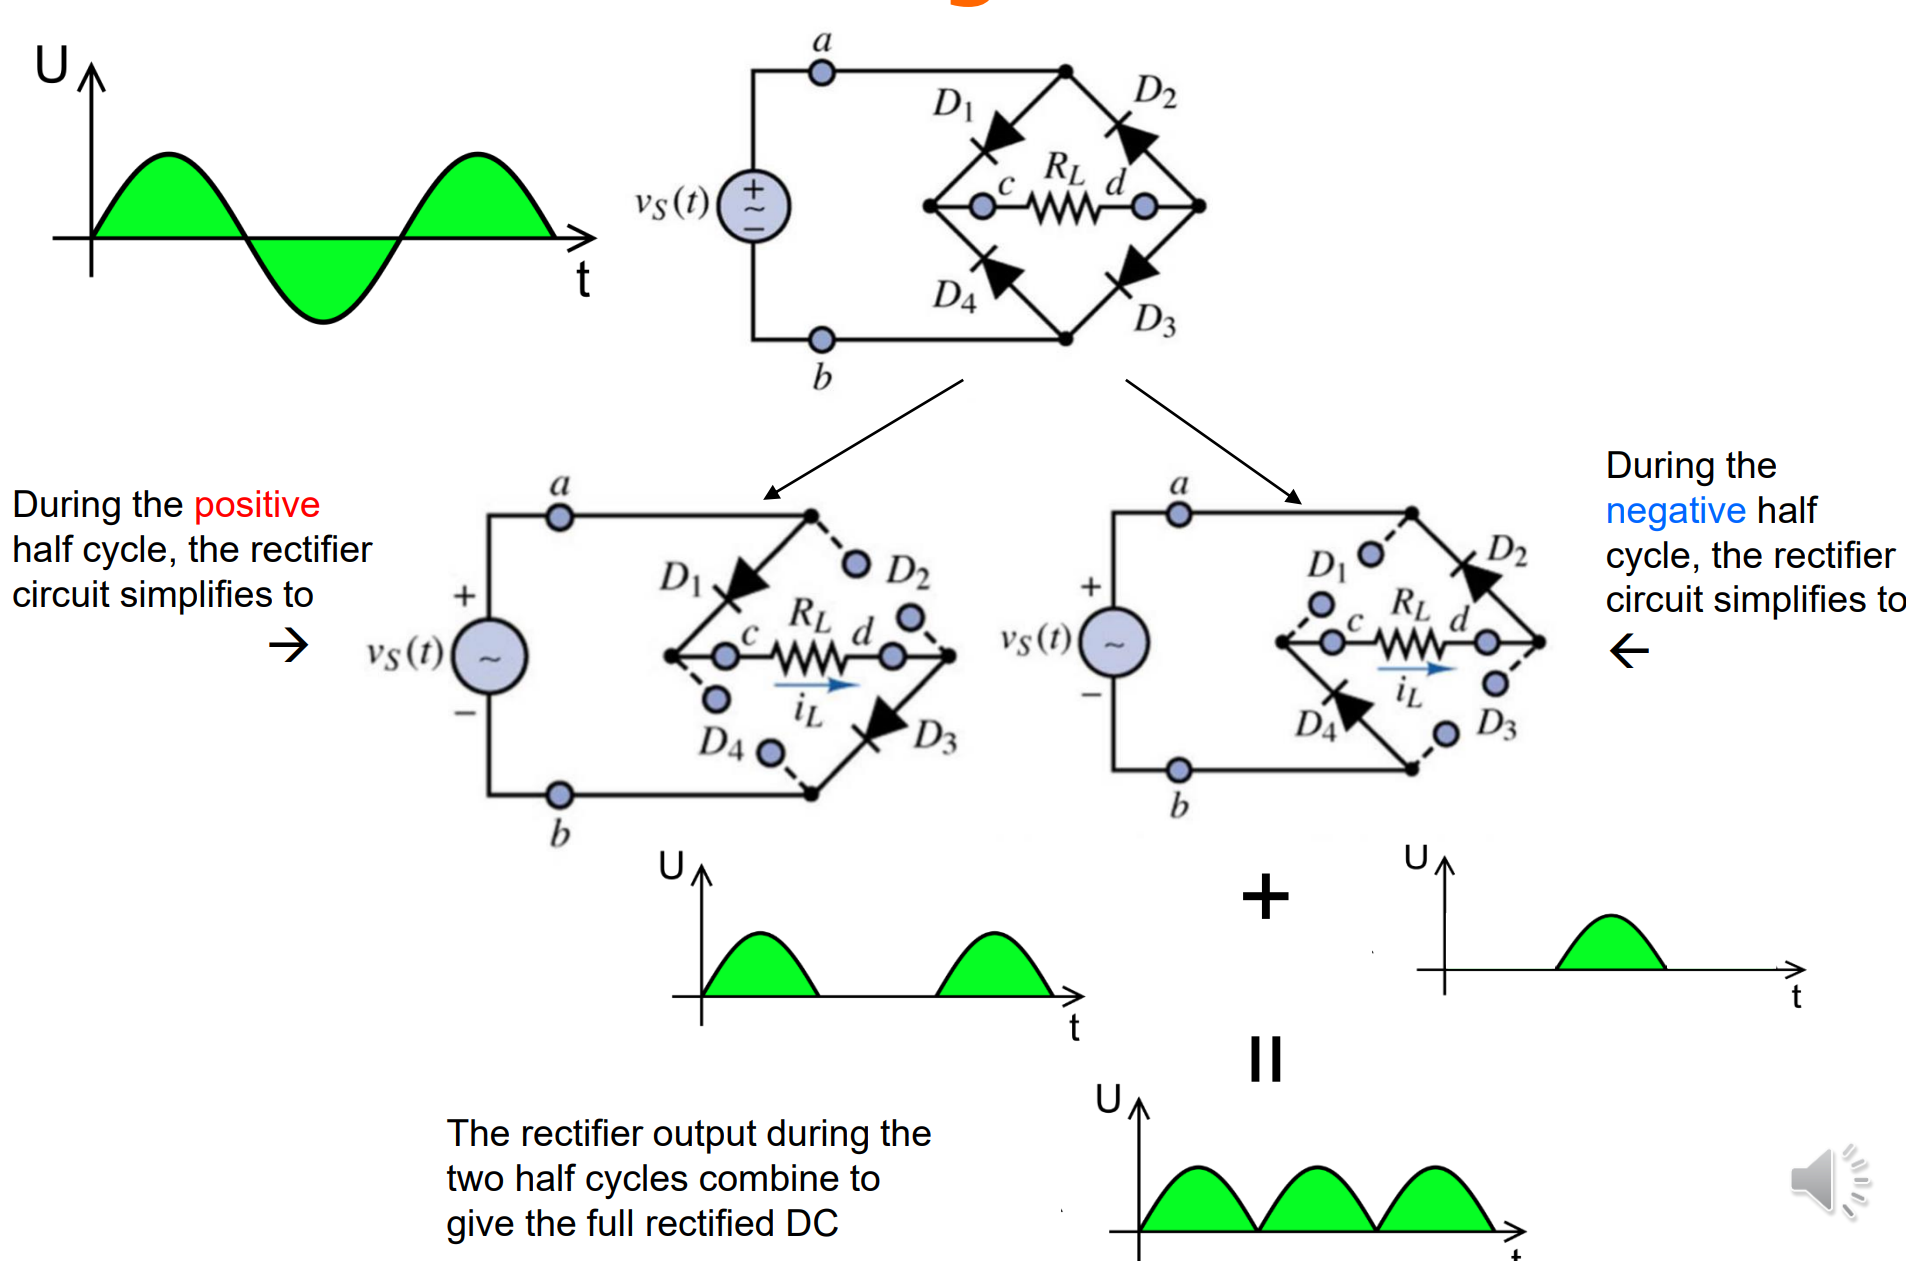
\includegraphics[width=0.9\linewidth]{images/diode-bridge-rectifier.png}}
    \item (\textbf{Voltage Ripple}) \\
    \centerline{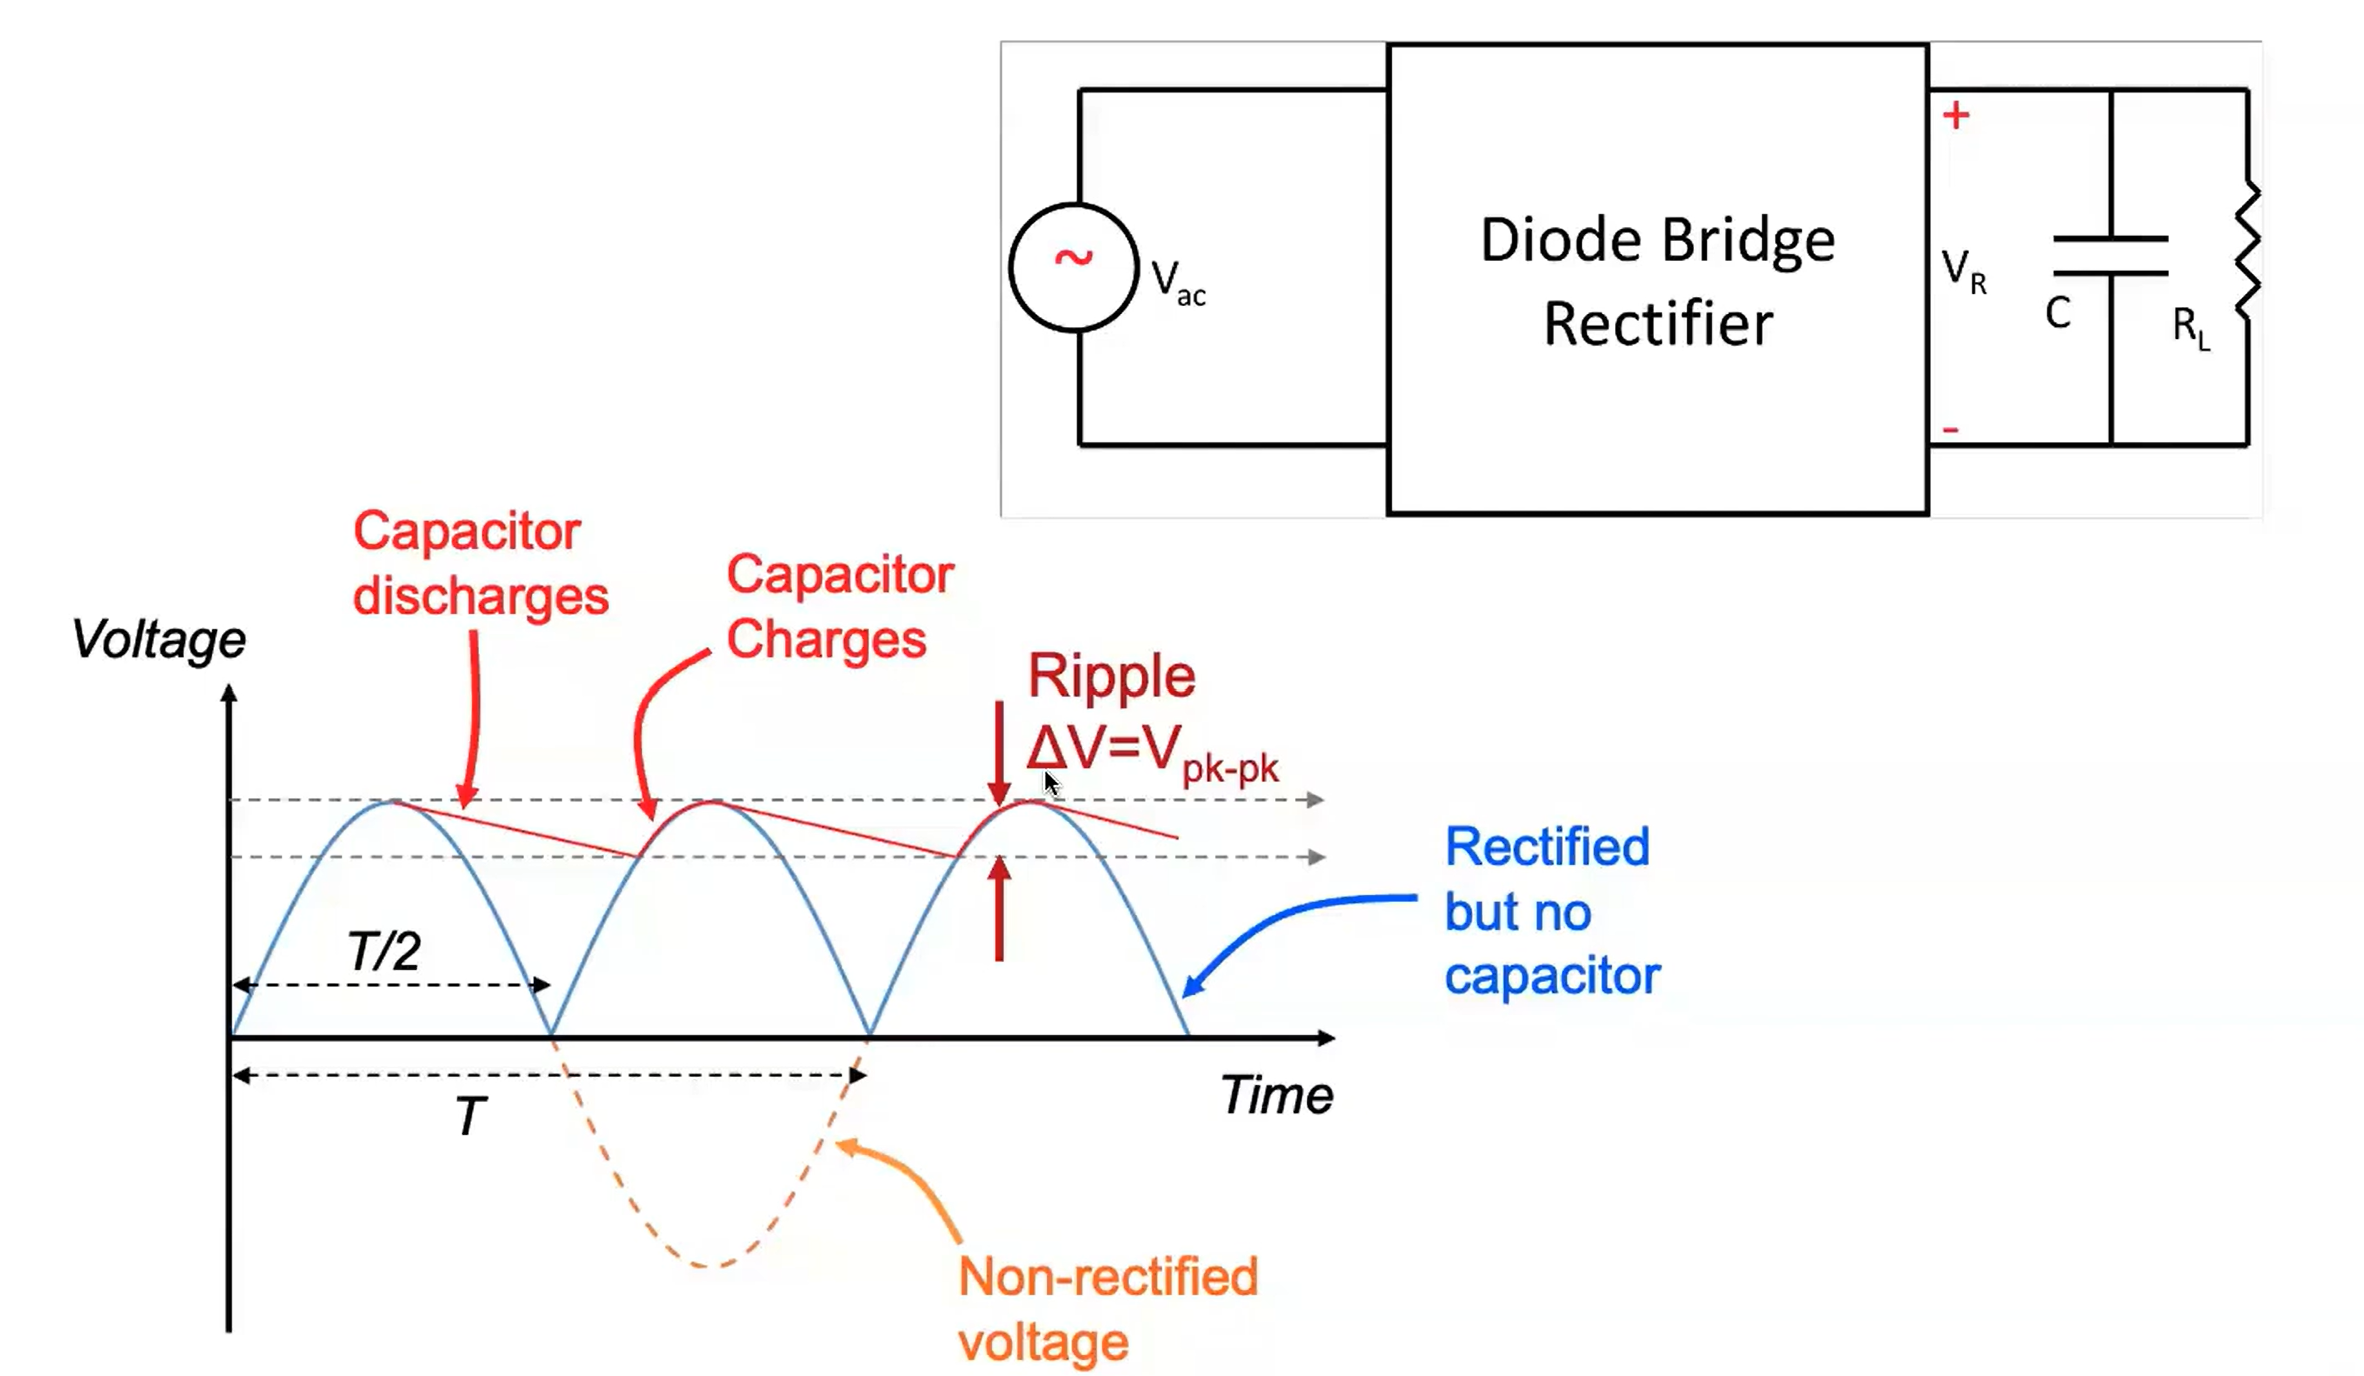
\includegraphics[width=0.9\linewidth]{images/voltage-ripple.png}}
    Using calculus, we can get $\Delta V \approx \frac{V_{\text{Load}}}{R_L}\times \frac{1}{2f_s} \times \frac{1}{C}$ ($V_{\text{Load}}$ is just $V_L$ here). Note that
    \begin{itemize}
        \item \textbf{The unit for $f$} should be in \textbf{Hz}. The formula to convert rad/s to Hz is $f=\omega / 2\pi$.
        \item Sometimes $\frac{V_{\text{Load}}}{R_L}$ is given as \textbf{current}.
    \end{itemize}
    \item (\textbf{LED}) LED is an application of diodes and when designing circuits
    \begin{itemize}
        \item Use Diode symbol to represent LEDs and write the LED's color just beside the symbol
        \item Add a resistor (usually is $330\Omega$ or $560\Omega$ and in the unit of several hundreds $\Omega$) in series with the LED for safety concerns.
    \end{itemize}
    \item (\textbf{Application of Forward/Backward Biased LED}) In the circuit below, using the characteristic of forward biased and backward biased diode, we can achieve the effect that when the output voltage from the comparator is positive, only LED1 will be lit up. If it is negative, only LED2 will be lit up. \\
    \centerline{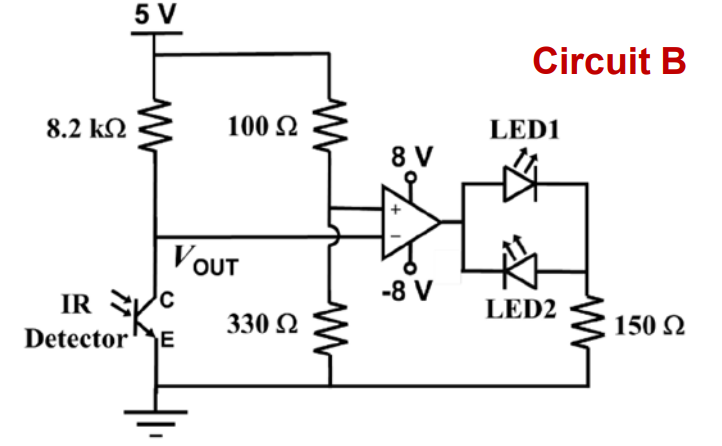
\includegraphics[width=0.7\linewidth]{images/biased-led-application.png}}
\end{enumerate}

\section{02. (Studio 8) DC Motors}
\begin{enumerate}
    \item (\textbf{Characteristics}) The stationary part in a motor is called \textbf{stator}, and the moving part is called \textbf{rotor}. In CG1111A, we only deal with permanent magnet DC (PMDC) motor.
    \item (\textbf{Motor Speed}) Motor speed is often specified as \textbf{RPM}(revolutions per minute). The relation between RPM and angular speed $\omega$ is $\omega=2\pi \times \frac{\text{RPM}}{60} \text{[rad/s]}$
    \item (\textbf{Motor Constant $K_t$}) Torque produced is proportional to motor current $I_m$, $T_{\text{shaft}}=K_tI_m \text{ [N.m]}$. $K_t$ is called \textbf{torque constant} and
    \begin{itemize}
        \item It describes how well the motor \textbf{converts current into torque}
        \item Depends on \textbf{magnetic properties} and \textbf{geometry} of motor
        \item Normally measured after motor was built
    \end{itemize}
    \item (\textbf{Motor Constant $K_e$}) When a motor shaft spins, the \textbf{magnetic} flux passing through the rotor coil \textbf{changes}. The changing flux \textbf{induces an electromotive force} (emf) in the coil according to the faraday's law, which opposes the source current. The induced emf is called \textbf{back emf}, and is proportional to \textbf{rotational speed}: $E_b=K_e\omega \text{ [V]}$. $K_e$ is called \textbf{back emf constant} and it
    \begin{itemize}
        \item depends on \textbf{magnetic properties} and \textbf{geometry} of motor
        \item For PMDC Motor, $K_t=K_e$
    \end{itemize}
    \item (\textbf{Power})
    \begin{itemize}
        \item \textbf{Mechanical Power} at motor shaft $P_{\text{mech}}=T_{\text{shaft}}~\omega \text{ [W]}$
        \item \textbf{Electrical Power} supplied to motor: $P_{\text{in}}=V_mI_m \text{ [W]}$
    \end{itemize}
    \item (\textbf{Motor Efficiency}) The \textbf{Efficiency} of motor is $\eta=\frac{P_{\text{out}}}{P_{\text{in}}}$. The mechanical power available at shaft is always \textbf{less than} electrical power input.
    \item (\textbf{Circuit Representation of PMDC Motor})
    \begin{itemize}
        \item From the circuit $I_m=\frac{V_m-E_b}{R_m}$ (By using ohm's law on resistor $R$)
        \item Since $E_b=K_e\omega$, we have $I_m=\frac{V_m}{R_m}-\frac{K_e\omega}{R_m}$
    \end{itemize}
    \centerline{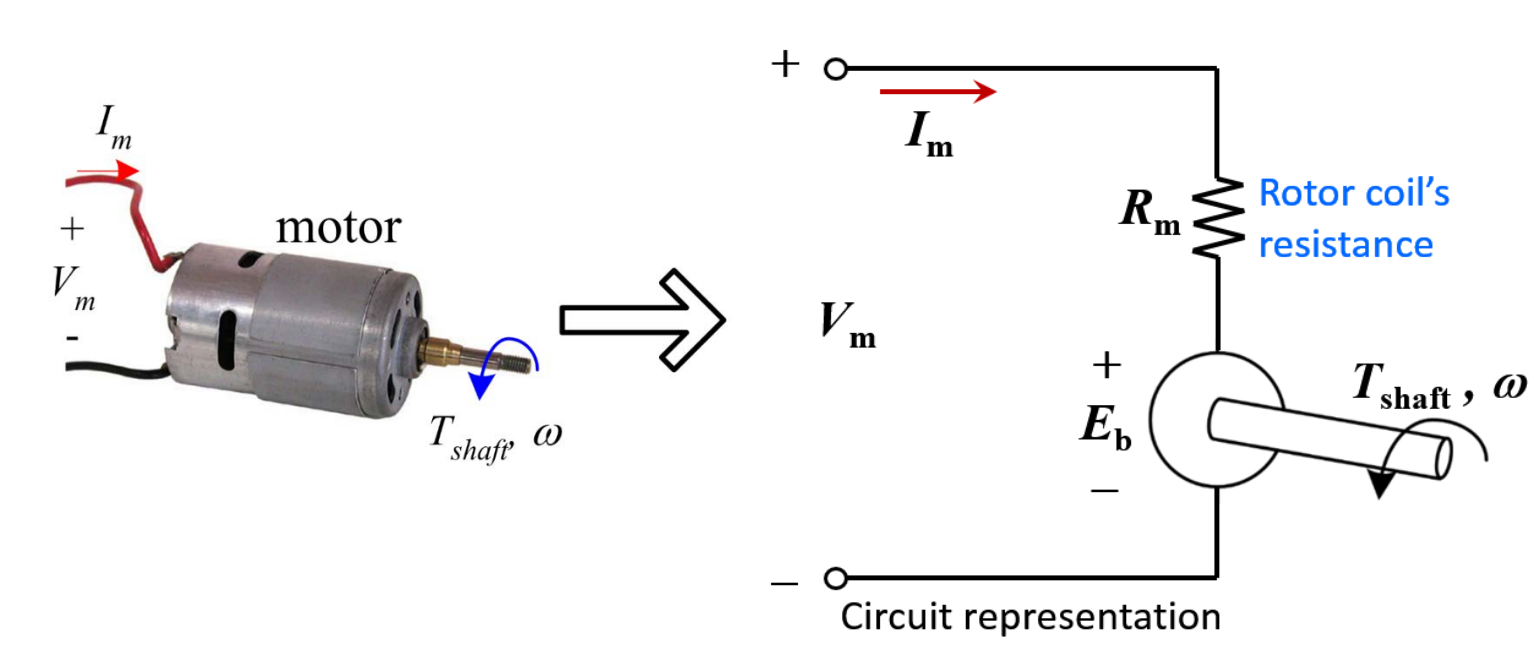
\includegraphics[width=0.9\linewidth]{images/circuit-representation-PMDC-motor.png}}
    \item (\textbf{Basic Properties of PMDC Motors}) Rearranging the $I_m$ formula above, we have $\omega = \frac{V_m}{K_e}-\frac{R_mI_m}{K_e}$
    \begin{itemize}
        \item For a \textbf{fixed-load} (i.e., \textbf{fixed $T_{\text{shaft}}$}, which implies \textbf{fixed $I_m$} since $T_{\text{shaft}}=K_tI_m$). This indicates that \textit{Shaft speed $\omega$ can be increased by increasing motor voltage $V_m$}.
        \item For a \textbf{fixed voltage $V_m$}, if $T_{\text{shaft}}$ increases, $I_m$ increases, and hence $\omega$ decreases. This indicates that \textit{shaft speed $\omega$ will be decreased with increasing load $T_{\text{shaft}}$}
    \end{itemize}
    \item (\textbf{Key parameters in Datasheet})
    \begin{itemize}
        \item (\textbf{No-load speed}) Speed at which shaft spins without mechanical load. (In the test, it means $I_m=0$, thus if we also know $V_m$, we can have our $K_e=V_m/\omega$)
        \item (\textbf{No-load current}) Current drawn under no-load speed. (In the test, it is 0) Note that when no load is attached to the motor shaft, the motor is still required to produce torque to overcome the \textbf{friction torque}.
        \item (\textbf{Stall torque}) Amount of load that causes the motor to stop ($\omega = 0$). This is the \textbf{maximum torque} the motor can produce. (In the test, it means $\omega=0$, thus $E_b=0$. So, we have $I_m=V_m/R_m$. Assuming that we know $K_e$ and $V_m$ already. Use this formula $T_{\text{shaft}}=K_e\cdot I_m$, since we already know $T_\text{shaft}$ also, it is just the Stall torque. Solve for $I_m$ first, then we can solve for our $R_m$)
        \item (\textbf{Stall current}) Current drawn under stall condition. Most motors will be \textbf{damaged} if subjected to \textbf{stall} conditions for \textbf{too long}.
    \end{itemize}
    \item (\textbf{Tips for solving DC Motor Problems})
    \begin{itemize}
        \item Don't chop in the problems first, try to find the motor's $K_e$ and $R_m$ first using the information given!
        \item After knowing these two important parameters. We can use our formula above to solve the problems.
        \item (\textbf{Some \textit{valueable} information hidden in the question})
        \begin{itemize}
            \item \textbf{load condition unchanged} means $I_m$ remains unchanged.
            \item \textbf{Power loss in rotor coil} means $\text{Electrical Power} - \text{Mechanical/Shaft Power}$, which is also the same as $P_{\text{loss}}=I_m^2*R_m$
        \end{itemize}
        \item In the question where the given $V_m, \omega, I_m(\text{torque})$ are changing, we \textbf{cannot} use the graph method to find $K_e$ by calculating the line's gradient and use the intercept with y-axis to find $R_m$! The \textbf{correct} way is to \textbf{plug in the given numbers and solve the equations!}
        \item Only when one of $V_m, \omega, I_m(\text{torque})$ is fixed can we use the gradient of the line to calculate $K_e$ and the y-intercept to calculate $R_m$.
    \end{itemize}
\end{enumerate}

\section{03. (Studio 9) Operational Amplifiers}
\begin{enumerate}
    \item (\textbf{What is an \textit{op-amp}}?)
    \begin{itemize}
        \item An \textit{operational amplifier (\textbf{op-amp})} is an integrated circuit that can amplify weak electric signals.
        \item It has \textbf{two input} signal terminals and \textbf{one output} signal terminal.
        \item It amplifies and outputs the \textbf{voltage difference} between the two input terminals.
    \end{itemize}
    \item (\textbf{Op-Amp Equivalent Circuit})
    \begin{itemize}
        \item $A$ is the open-loop voltage gain (It is very large, approaching $\infty$)
        \item $R_{\text{in}}$ is the input impedance (very large) and $R_{\text{out}}$ is the output impedance (very small)
        \item To \textbf{simplify} analysis, we always assume \textbf{infinite} $R_{\text{in}}$ and $A$, and $zero$ $R_{\text{out}}$
    \end{itemize}
    \centerline{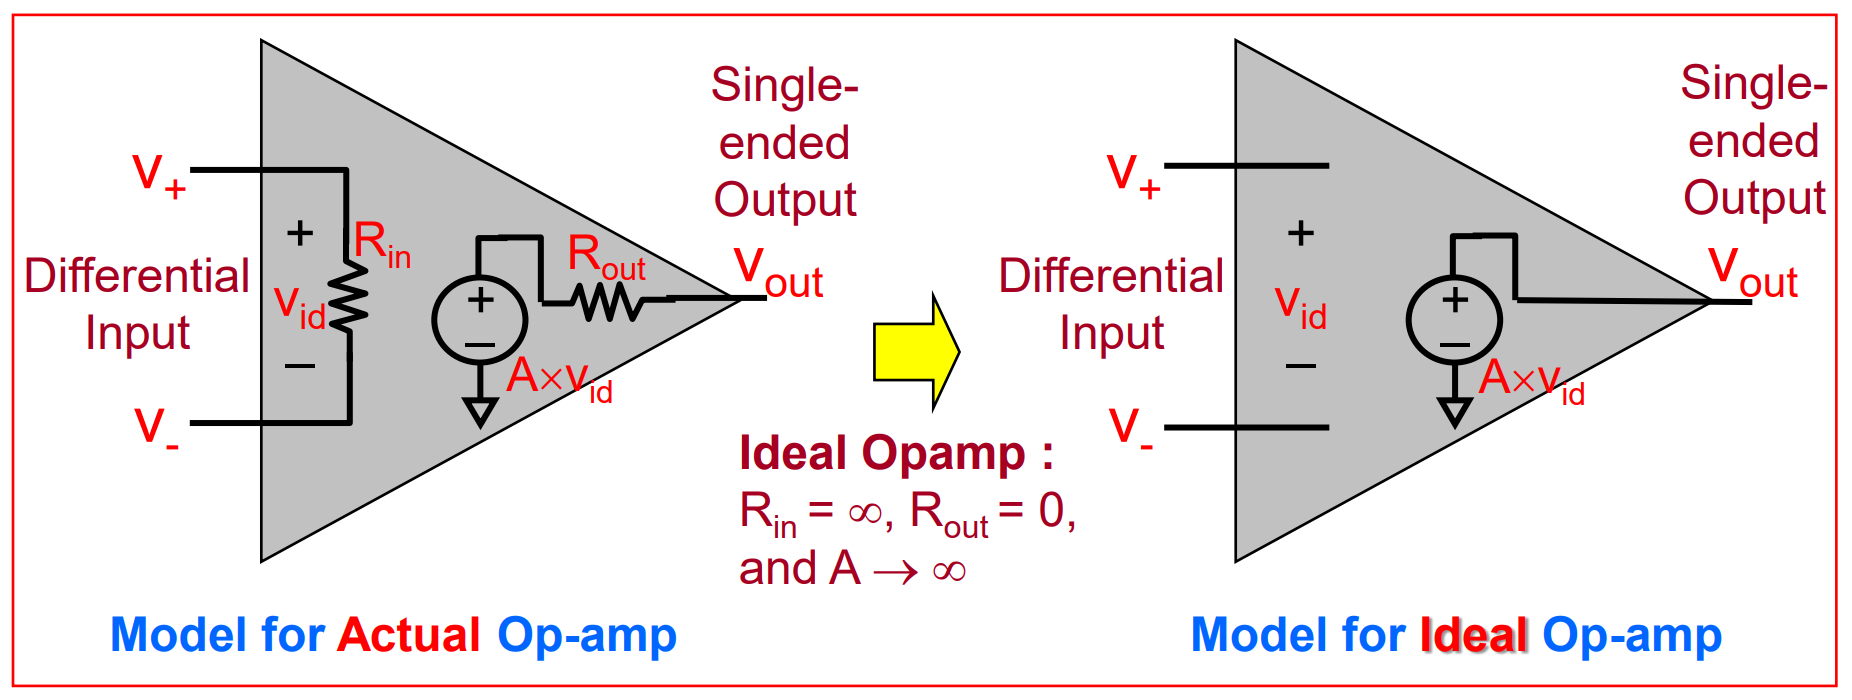
\includegraphics[width=0.9\linewidth]{images/op-amp-equivalent-circuit.png}}
    \item (\textbf{Op-amp Golden Rules})
    \begin{itemize}
        \item (\textbf{Rule 1}) \textbf{In a closed loop with -ve feedback}, the output attempts to do whatever is necessary to make the \textbf{voltage difference} between the \textbf{inputs zero}. This actually means \textbf{Virtual short}, i.e., $V_+\approx V_-$
        \item (\textbf{Rule 2}) The \textbf{inputs} draw \textbf{no current}. That means the current drawn at two inputs are zero.
    \end{itemize}
    \centerline{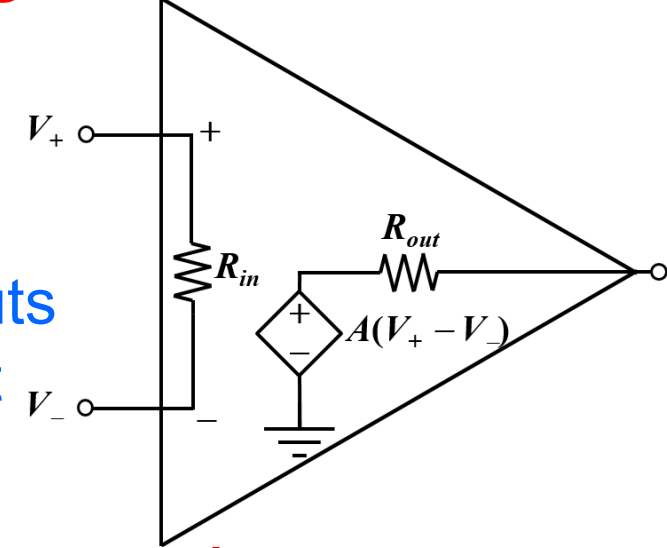
\includegraphics[width=0.5\linewidth]{images/op-amps-golden-rules.png}}
    \item (\textbf{Closed Loop}) There is connection between output and input.
    \item (\textbf{-ve feedback}) The output is fed back to the input in such a way to \textbf{reduce} the \textbf{output fluctuations}. \\
    \centerline{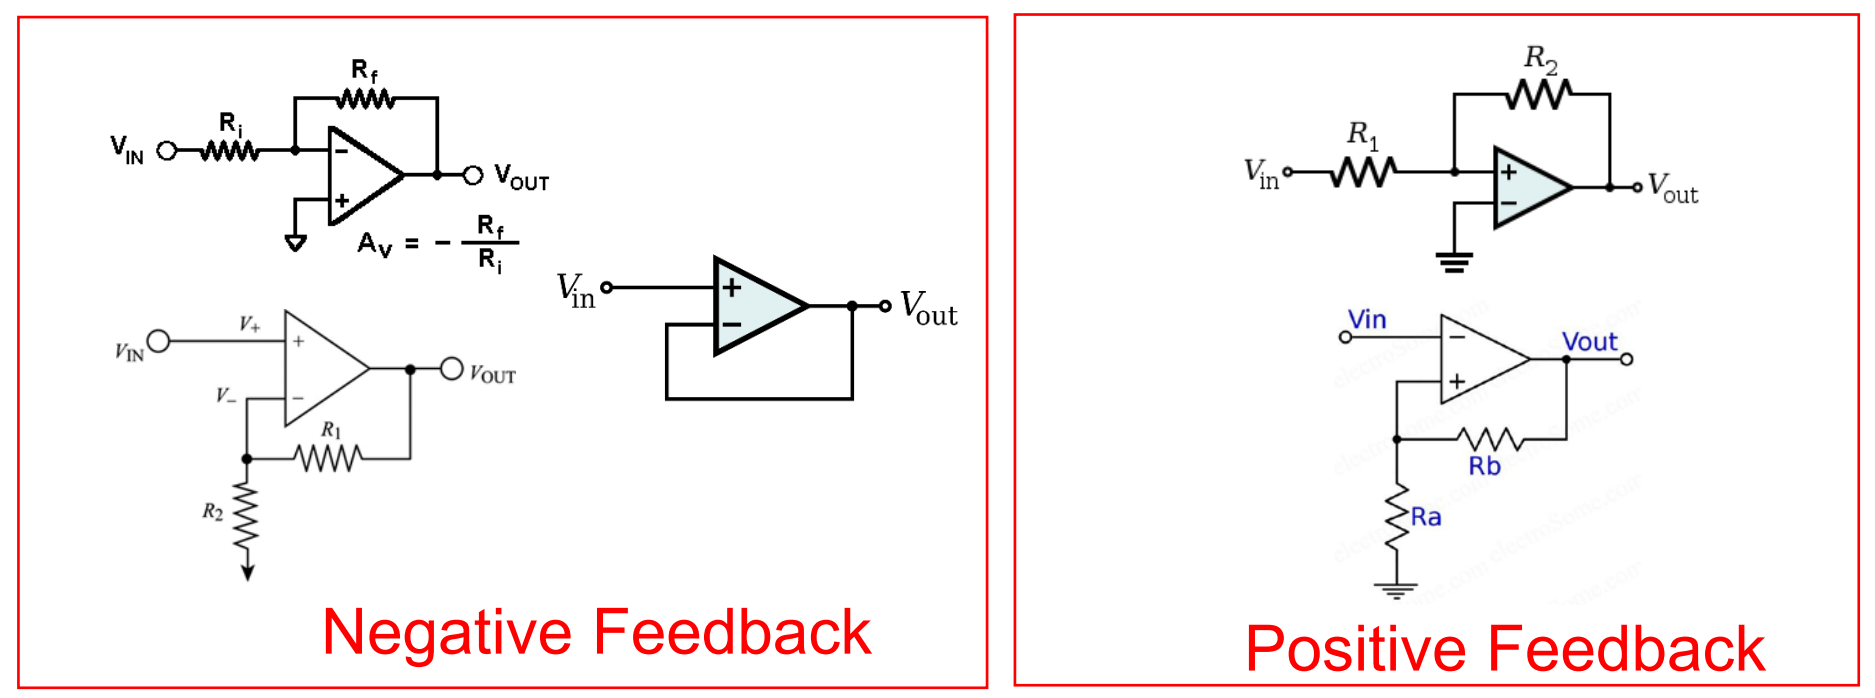
\includegraphics[width=1.0\linewidth]{images/posivite-negative-feedback.png}}
    \item (\textbf{Two Types of Amplifiers})
    \begin{itemize}
        \item (\textbf{Inverting Amplifier}) $\frac{v_{\text{out}}}{v_{\text{in}}}=-\frac{R_f}{R_i}$ \\
        \centerline{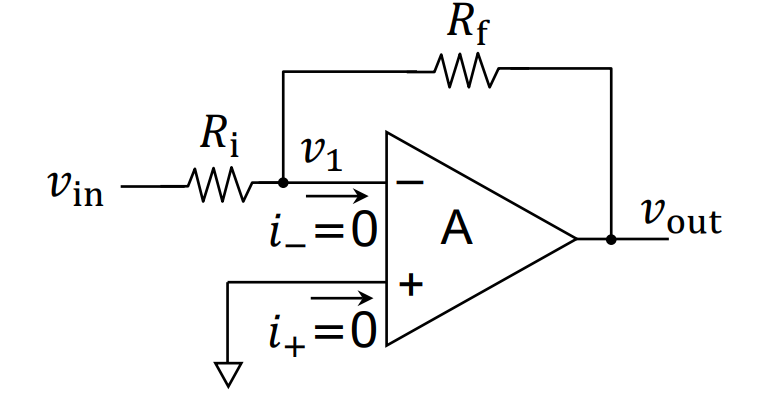
\includegraphics[width=0.6\linewidth]{images/inverting-amplifier.png}}
        \item (\textbf{Non-inverting Amplifier}) $\frac{v_{\text{out}}}{v_{\text{in}}}=1+\frac{R_f}{R_i}$ \\
        \centerline{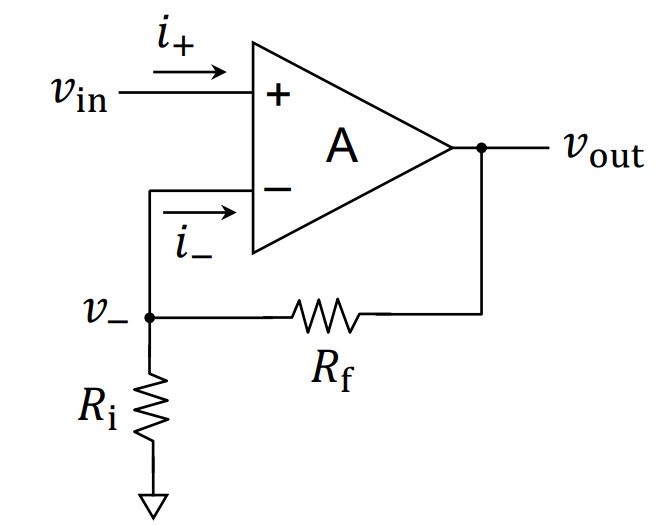
\includegraphics[width=0.5\linewidth]{images/non-inverting-amplifier.png}}
    \end{itemize}
    In real-world application/design (test), amplifier is used to amplify the signal (usually voltage) and the scaling factor is the \textbf{voltage gain} calculated in the formula above. So, what we should do is to find the proper ratio between $R_f$ and $R_i$ so that we can achieve that voltage gain. (\textbf{Usually for the voltage gain, we care about its magnitude} and the amplified $V_{\text{out}}$ is question-specific. If it is arduino, it will be 5V. Otherwise, it depends.)
    \item (\textbf{Permissible Resistor Range}) Rule of thumb: $R_i$ and $R_f$ should be within ($10 \times R_{\text{out, }}0.1 \times R_{\text{in}}$) \\
    \centerline{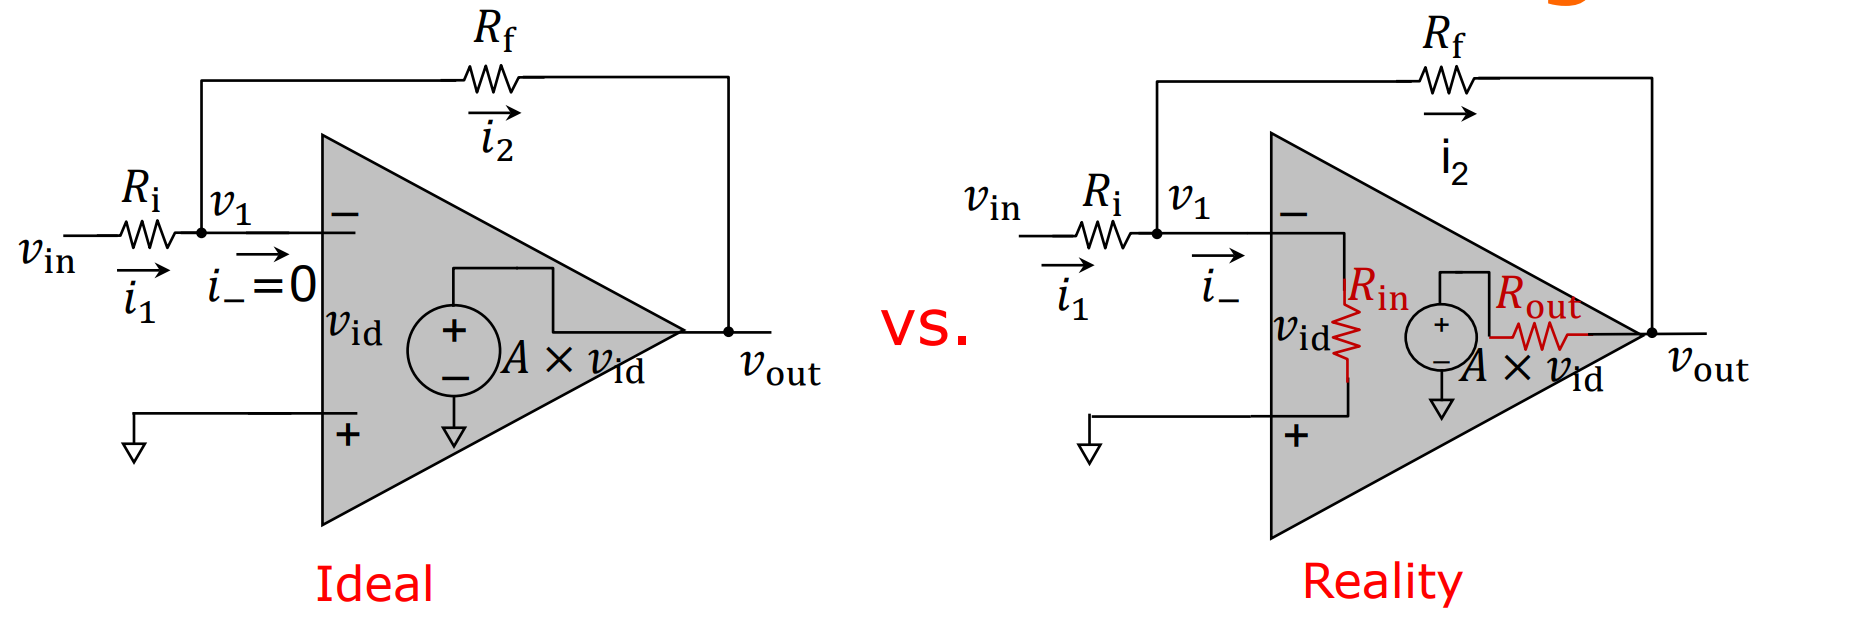
\includegraphics[width=0.9\linewidth]{images/permissible-resistor-range.png}}
    \item (\textbf{Positive vs Negative Gain})
    \begin{itemize}
        \item \textbf{Negative} gain \textbf{does not mean loss} (When you get a negative gain in the test, just leave it as it is)
        \item Negative gain only means output is the \textbf{inverted version} of input ($180^{\circ}$ phase shift)
        \item Only when gain magnitude is \textbf{less than 1}, there is \textbf{loss}
    \end{itemize}
    \centerline{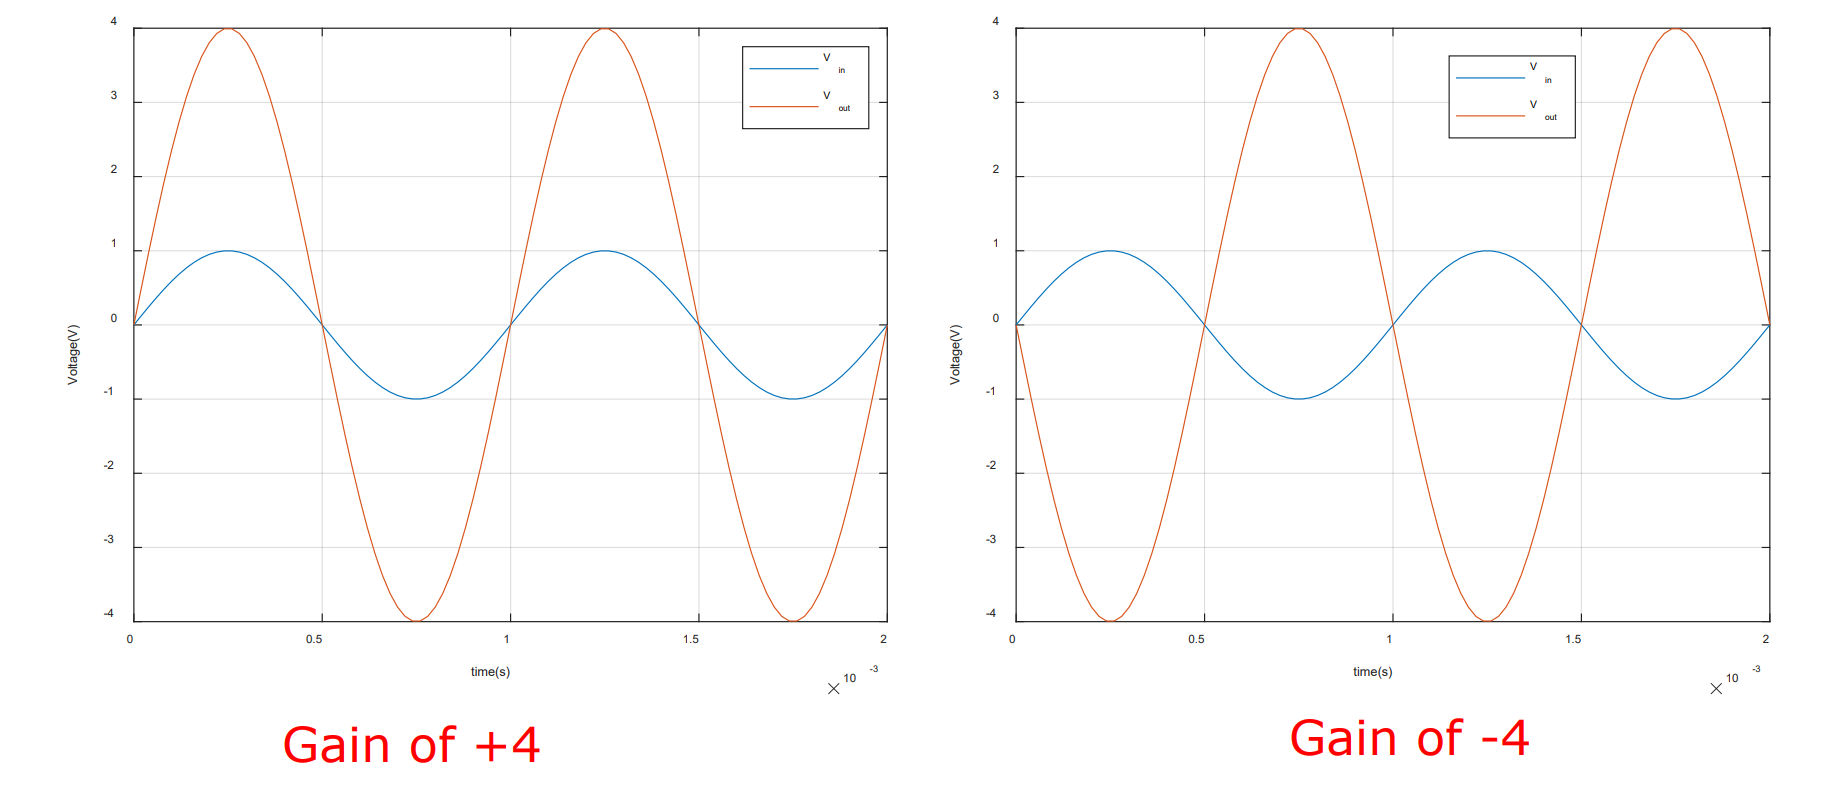
\includegraphics[width=0.9\linewidth]{images/positive-vs-negative-gain.png}}
    \item (\textbf{Solving Tips})
    \begin{itemize}
        \item When using KCL on amplifiers, try analysing the node that is the \textbf{input} to the amplifier since according to golden rule (2), one branch has \textbf{no current flowing}.
        \item Remember to use \textbf{potential divider} to calculate some node's voltage to save time.
    \end{itemize}    
\end{enumerate}

\section{04. (Studio 10) Op-amp Comparators \& Filters}
\subsection{Op-amp Comparators}
\begin{enumerate}
    \item (\textbf{What is an op-amp comparator?})
    \begin{enumerate}
        \item A \textbf{comparator} is an electronic device that can compare an \textbf{analog signal} with a \textbf{given threshold}, and produce a \textbf{digital output}.
        \item The \textbf{op-amp} comparator makes use of an op-amp's very high gain in its \textbf{open-loop state} (i.e., there is no \textbf{feedback resistor}, or basically, there is not closed loop!)
    \end{enumerate}
    \centerline{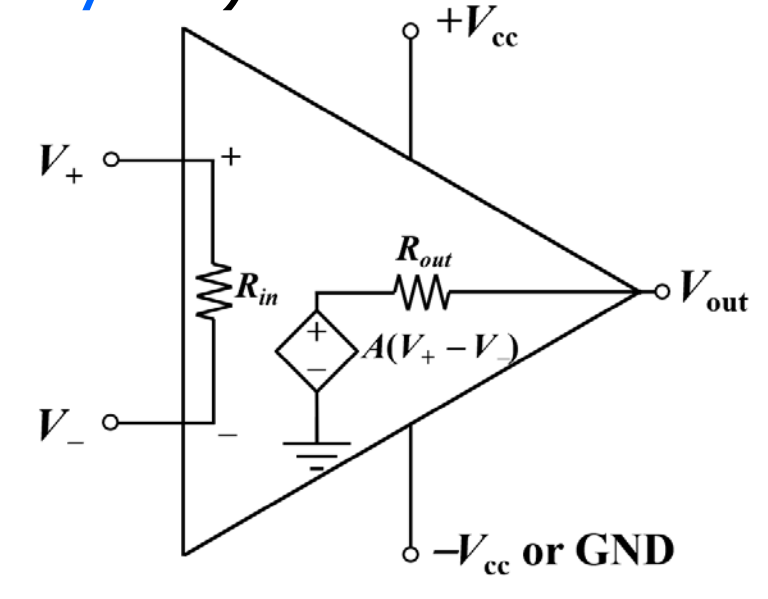
\includegraphics[width=0.5\linewidth]{images/comparator.png}}
    \item (\textbf{Saturation Voltage}) Basically, it is
    \begin{itemize}
        \item If $V_+>V_-$: $V_{\text{out}}=V_{\text{cc}}-V_{\text{ovh1}}$ or just $V_{\text{out}}=V_{\text{cc}}$
        \item If $V_+<V_-$: $V_{\text{out}}=\begin{cases}
            -V_{\text{cc}}+V_{\text{ovh2}} & \text{if \textbf{dual} power supply} \\
            V_{\text{ovh2}} & \text{if \textbf{single} power supply}
        \end{cases}$
        or just $V_{\text{out}}=\begin{cases}
            -V_{\text{cc}} & \text{if \textbf{dual} power supply} \\
            0 & \text{if \textbf{single} power supply}
        \end{cases}$
    \end{itemize}
    $V_{\text{ovh1}} \text{ and } V_{\text{ovh2}}$ are the \textbf{voltage headrooms} from the \textbf{supply rails} needed to sustain proper \textbf{output transistor} turn-on voltage. Usually we just ignore them in the test. \textbf{But the application about when the output is $V_{\text{cc}}$ and when the output is $V_0$ is important to our design!}
    \item (\textbf{Inverting vs. Non-Inverting Comparator})
    \begin{itemize}
        \item (\textbf{Non-Inverting Comparator}) Ideally, $V_{\text{out}}=A\times (V_{\text{in}}-V_{\text{REF}})$ \\
        \centerline{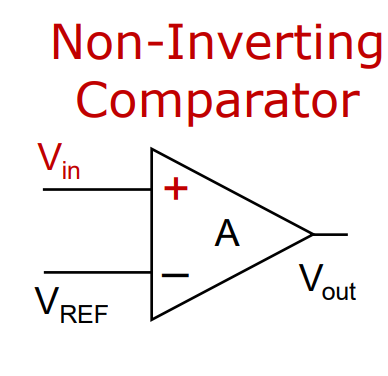
\includegraphics[width=0.3\linewidth]{images/non-inverting-comparator.png}}
        \item (\textbf{Inverting Comparator}) Ideally, $V_{\text{out}}=A\times (V_{\text{REF}}-V_{\text{in}})=-A\times (V_{\text{in}}-V_{\text{REF}})$ \\
        \centerline{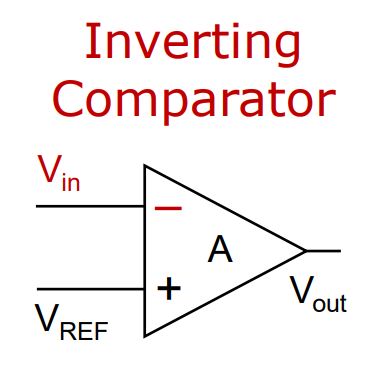
\includegraphics[width=0.3\linewidth]{images/inverting-comparator.png}}
        All in all, in the test, \textbf{we don't need to care about whether ther comparator is inverting/non-inverting}. All we need to care about is \textbf{whether the voltage coming in the + input is bigger than the voltage coming in - input}. If it is, the comparator will output $V_{\text{cc}}$, otherwise it will be $-V_{\text{cc}}$ (if dual power supply) or $0$ (if single power supply).
    \end{itemize}
\end{enumerate}

\subsection{Filters}
\begin{enumerate}
    \item (\textbf{What is filter?}) A filter is a device or process that \textbf{removes} some \textbf{unwanted components} or \textbf{features} from a signal.
    \item (\textbf{Passive Low-Pass Filter}) \textbf{Passive} means no op-amps are used in the circuit. \textbf{Low-pass} means only low frequency signal can pass.
    \begin{itemize}
        \item Capacitor impedance is given as $1/(j\omega C)$
        \item At low frequency, use $\omega = 2\pi / T=2\pi f$, we can see $\omega$ decreases, capacitor behaves like \textbf{open} circuit.
        \item Similarly, at high frequency, $\omega$ increases, capacitor behaves like \textbf{short} circuit.
    \end{itemize}
    \centerline{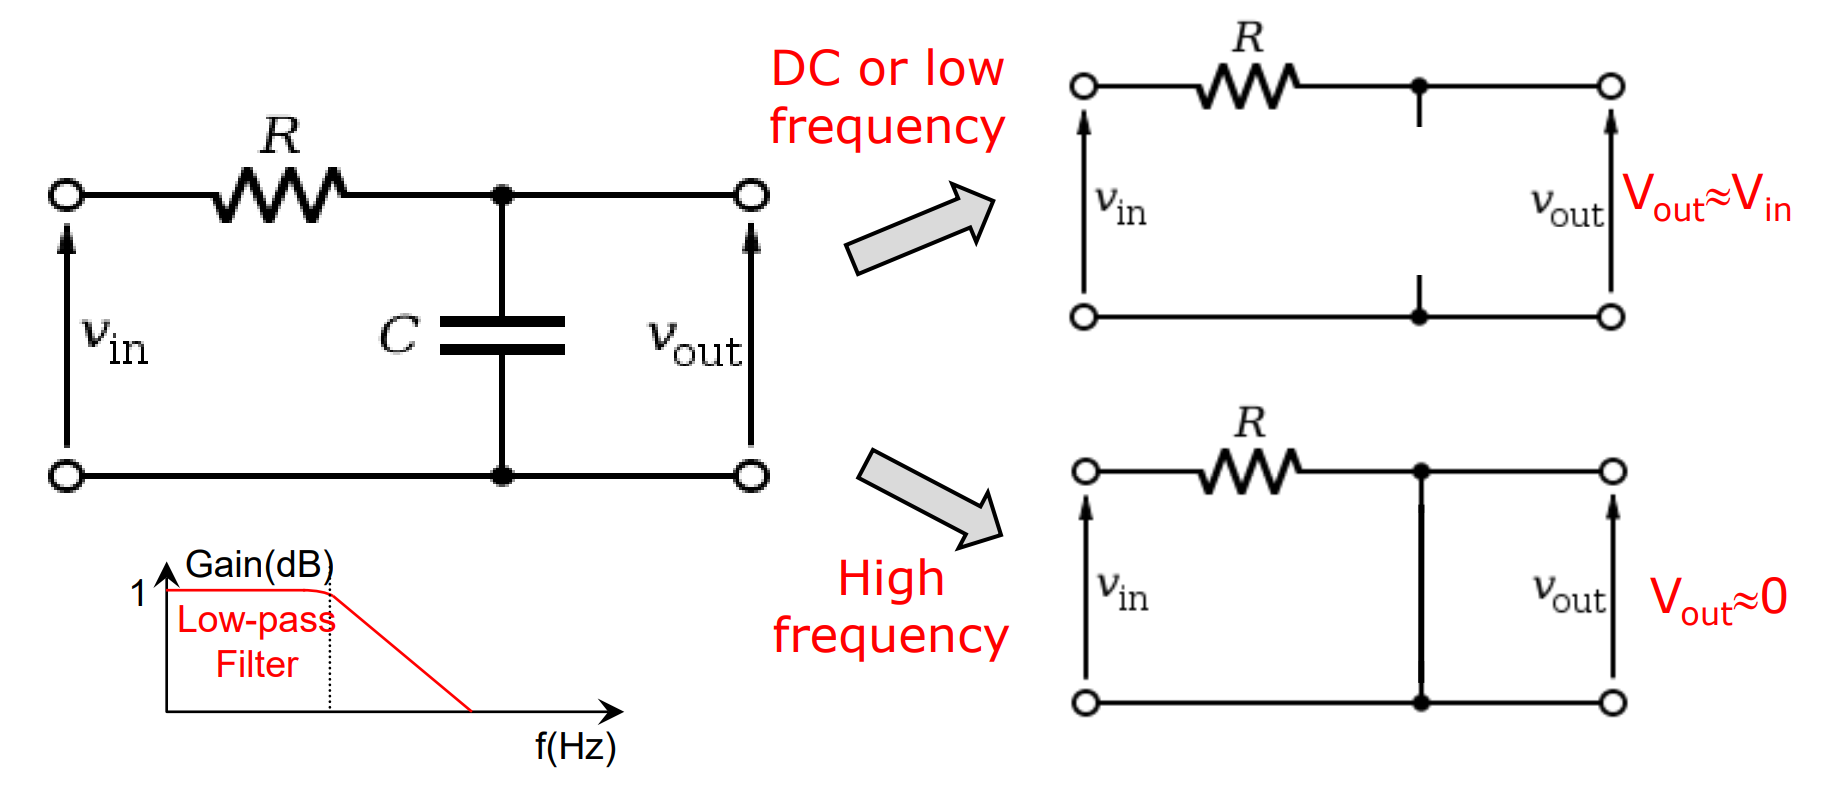
\includegraphics[width=0.9\linewidth]{images/passive-low-pass-filter.png}}
    \item (\textbf{Power/Voltage Gain in decibels(dB)})
    \begin{itemize}
        \item The \textbf{Voltage Amplification ($A_v$) or Gain} of a voltage amplifier/filter is given by $A_v=\frac{V_{\text{out}}}{V_{\text{in}}}$
        \item The voltage gain can also be commonly expressed in terms of the resulting \textbf{power gain} in \textbf{dB}: $\text{Power Gain (dB)}=20log_{10}|\frac{V_{\text{out}}}{V_{\text{in}}}|$ dB.
    \end{itemize}
    \item (\textbf{Cut-off Frequency}) The cut-off frequency characterizes a \textbf{boundary} between a \textbf{passband} (the range of frequencies that a filter allows to pass through with little or no attenuation) and a \textbf{stopband} (the range of frequencies that a filter significantly attenuates or blocks)
    \begin{itemize}
        \item It is defined as the frequency at which the \textbf{output power} is reduced by \textbf{half} compared to the nominal passband value.
        \item In \textbf{dB scale}, this is equivalent to the nominal passband value reduced by about 3dB. (Using $10log_{10}0.5$ to calculate).
        \item The cut-off frequency is a \textbf{property} of a filter. So, it is fixed as long as our $RC$ is fixed.
    \end{itemize}
    \item (\textbf{Method to find Cut-off Frequency})
    \begin{enumerate}
        \item Always find $\frac{V_{\text{out}}}{V_{\text{in}}}$ first
        \item Manipulate the formula above, manipulate the numerator to be 1 and then put all the $\omega$ terms in the denominator.
        \item Use the given sample point to calculate $RC$ of the filter. (The sample point is usually stated like suppressed at the 10kHz noise by 20dB, this means at frequency \textbf{10kHz}, the power gain in dB is reduced by \textbf{20dB}) 
        \item Use $f_c=\frac{1}{2\pi RC}$ to calculate the cut-off frequency
    \end{enumerate}
    Below are some examples, but the whole idea is listed above.
    \begin{itemize}
        \item (\textbf{Gain in dB of Passive Low-Pass Filter}) \\
        \centerline{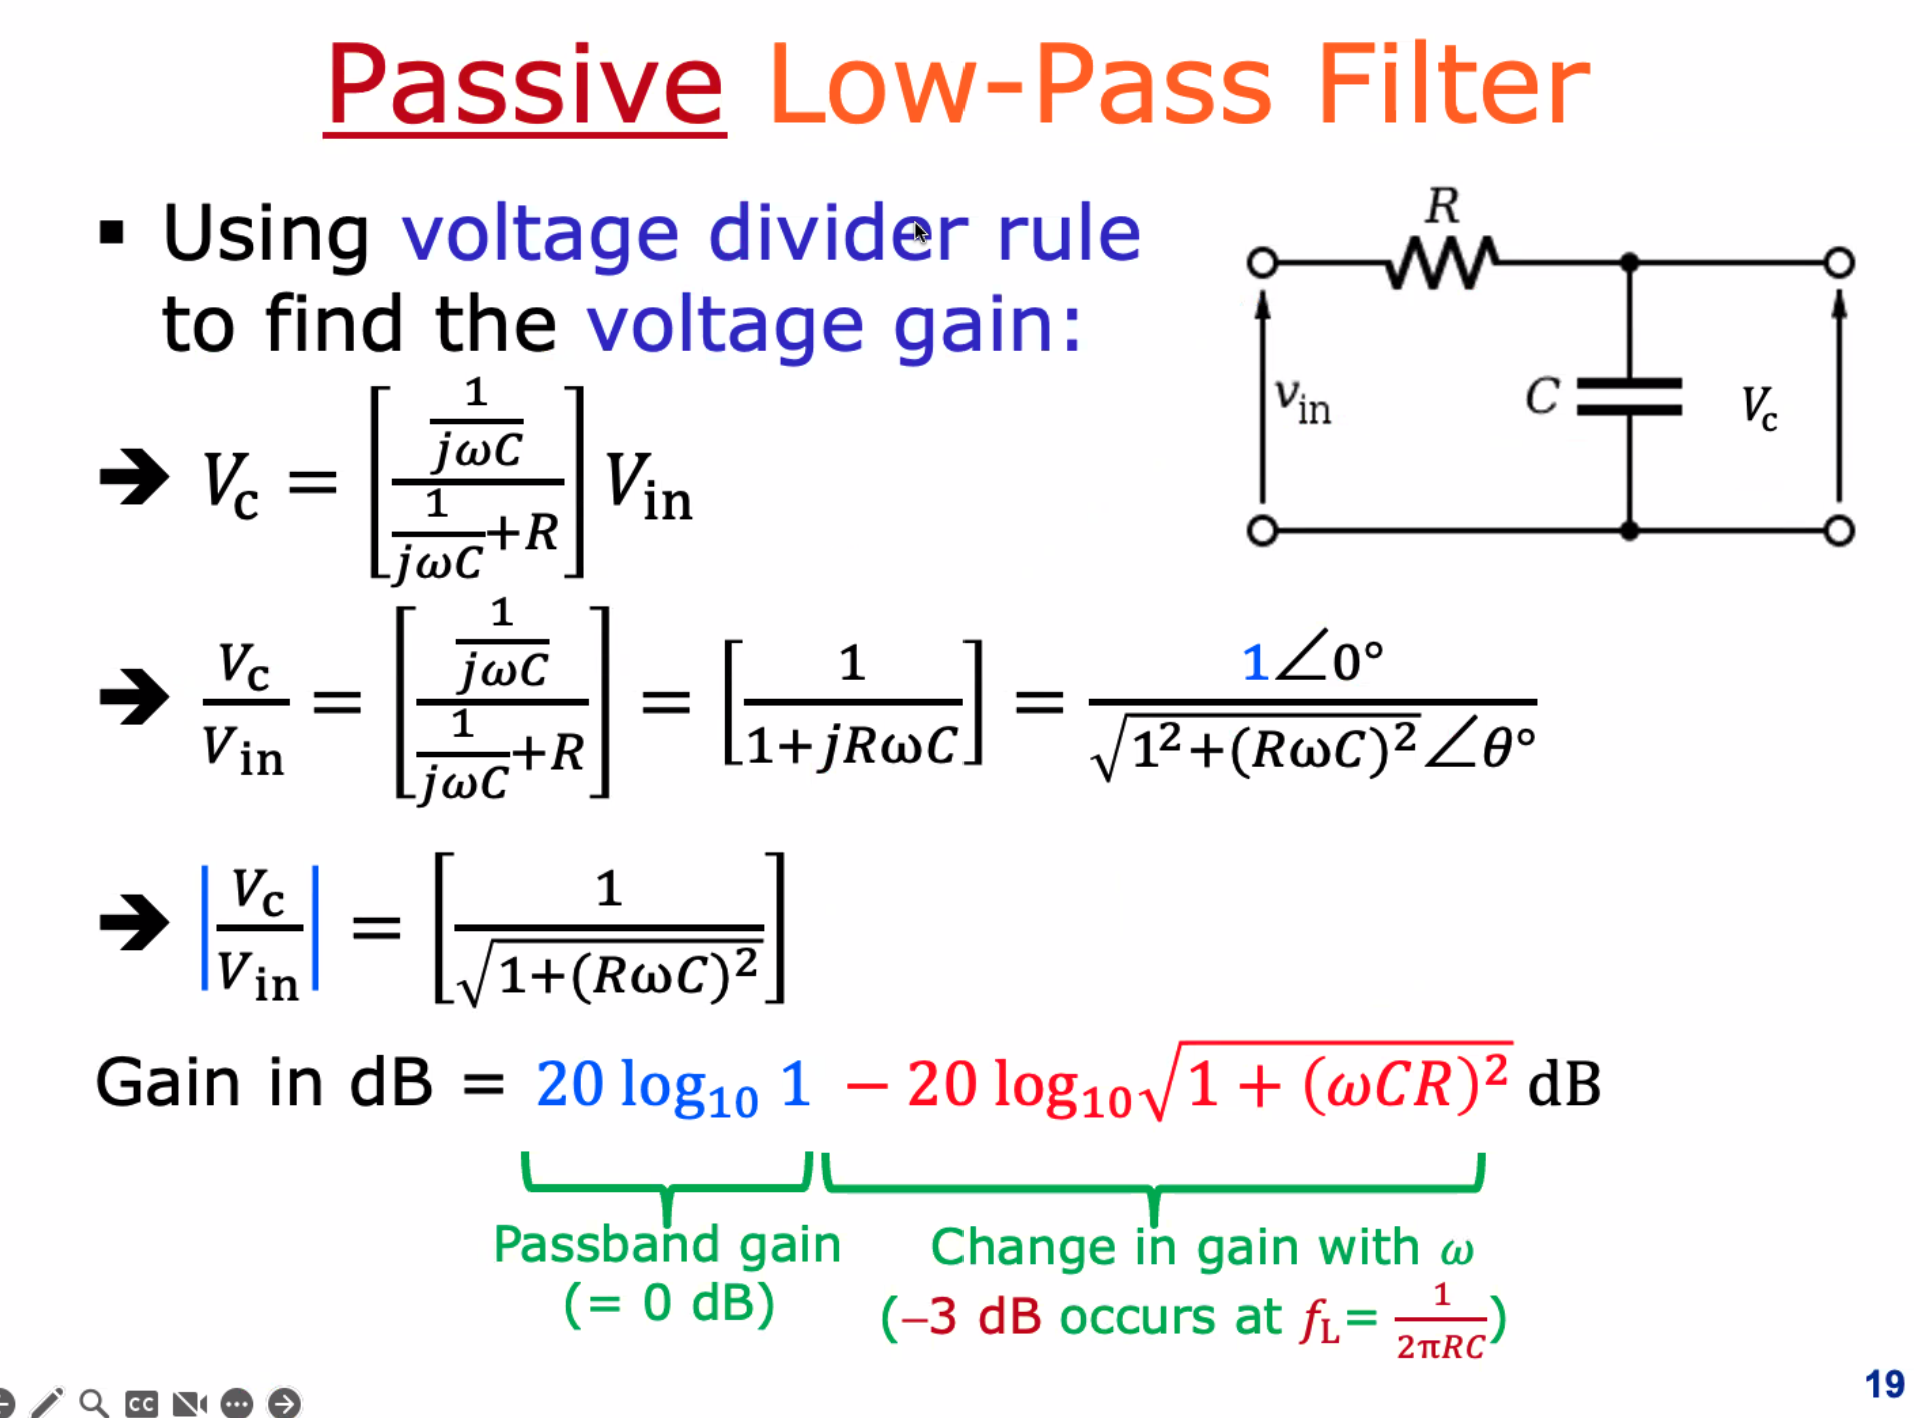
\includegraphics[width=0.9\linewidth]{images/gain-of-passive-low-pass-filter.png}}
        \item (\textbf{Gain in dB of Passive High-Pass Filter}) \\
        \centerline{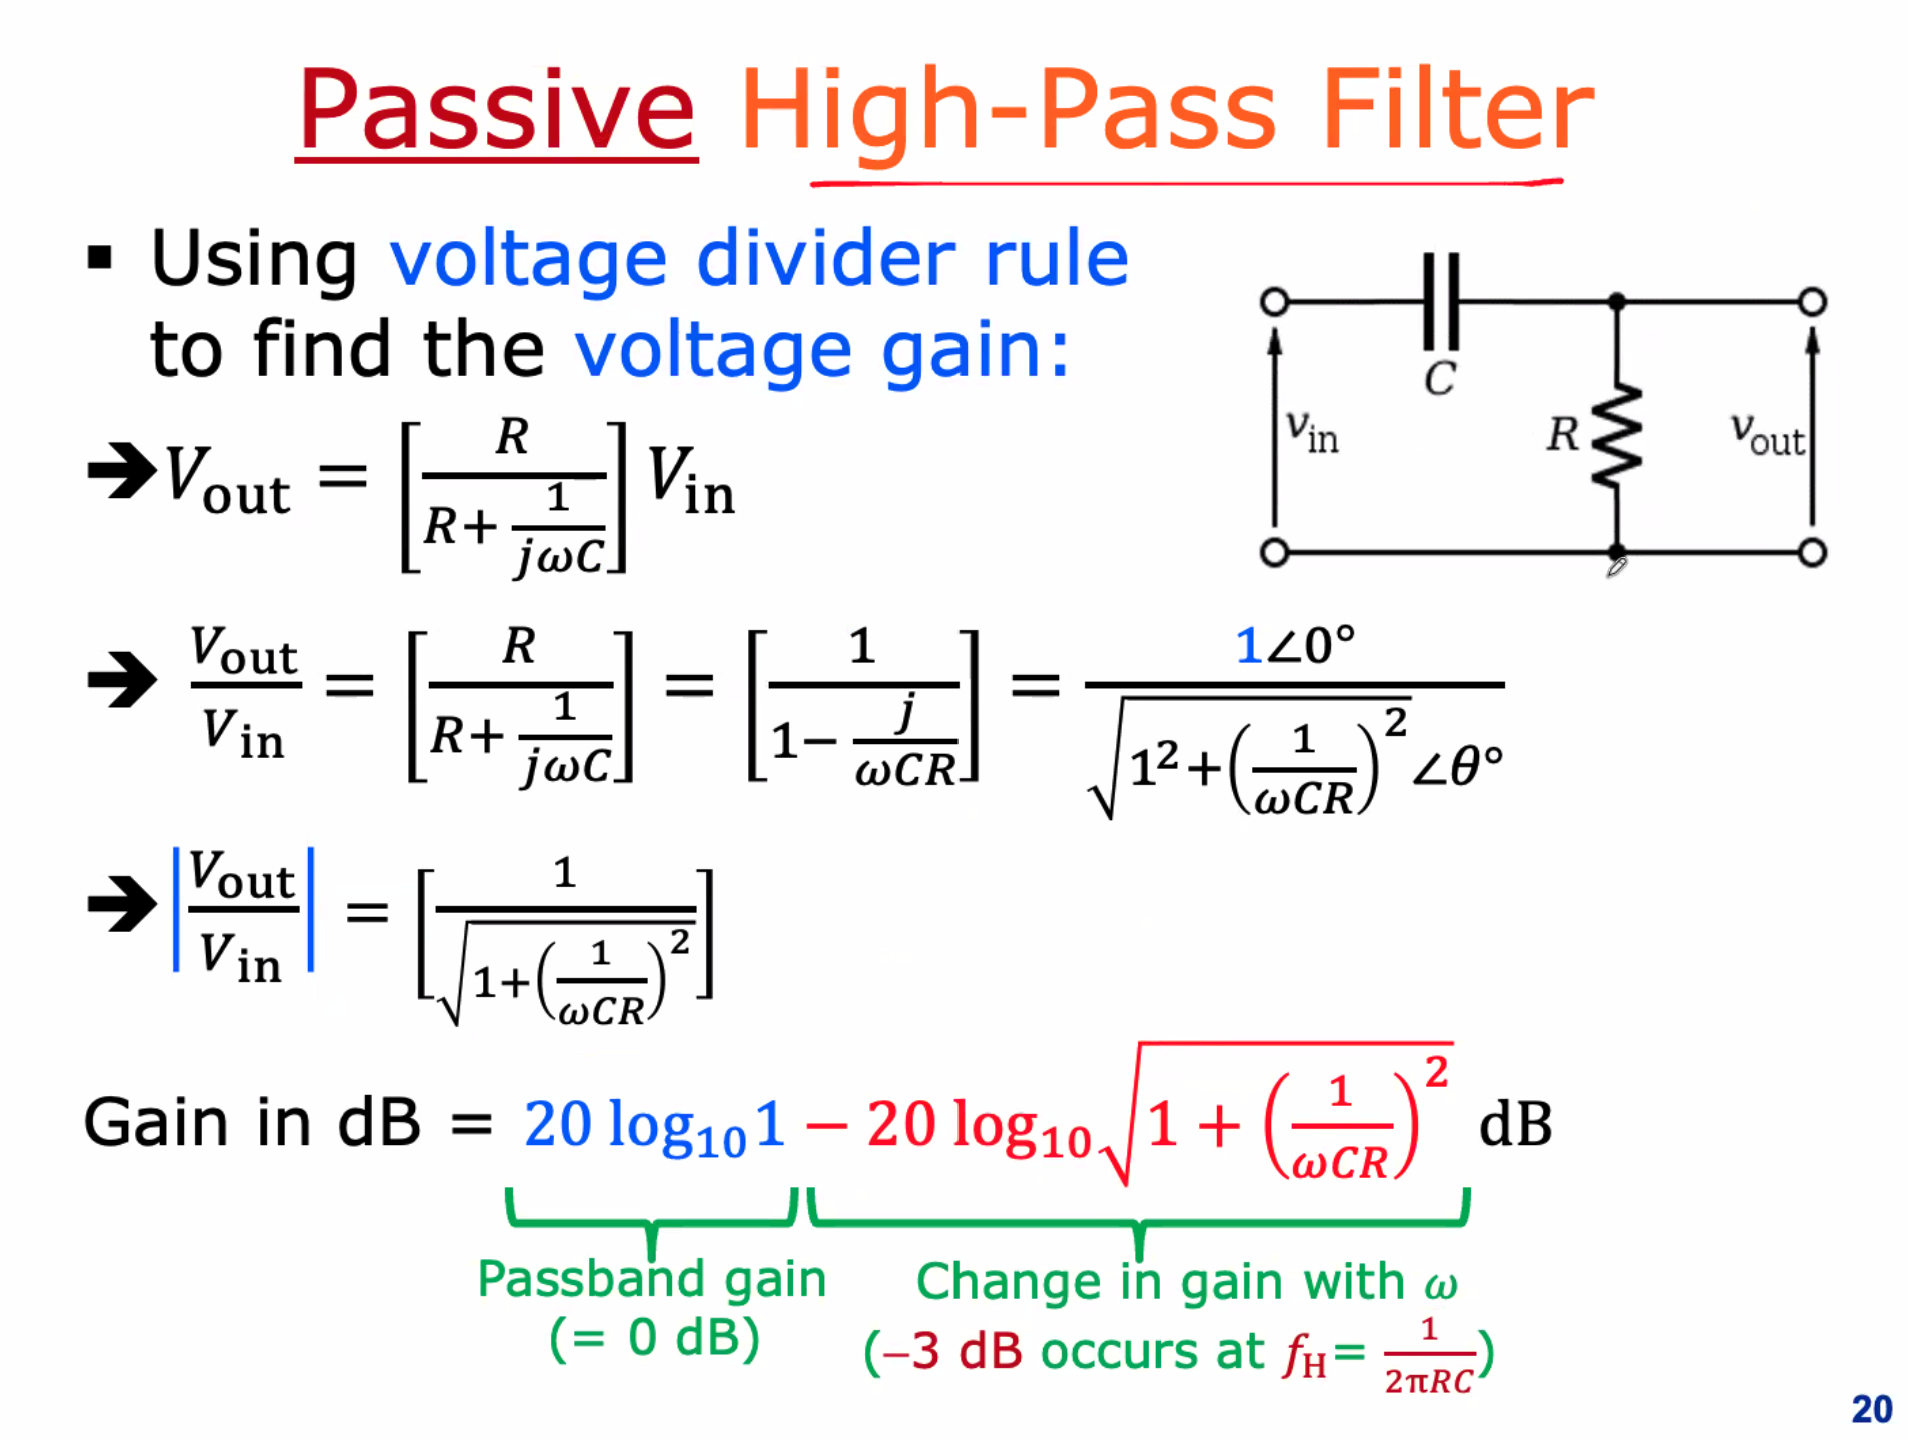
\includegraphics[width=0.9\linewidth]{images/gain-of-passive-high-pass-filter.png}}
        \item (\textbf{Gain in dB of Active Low-Pass Filter}) \\
        \centerline{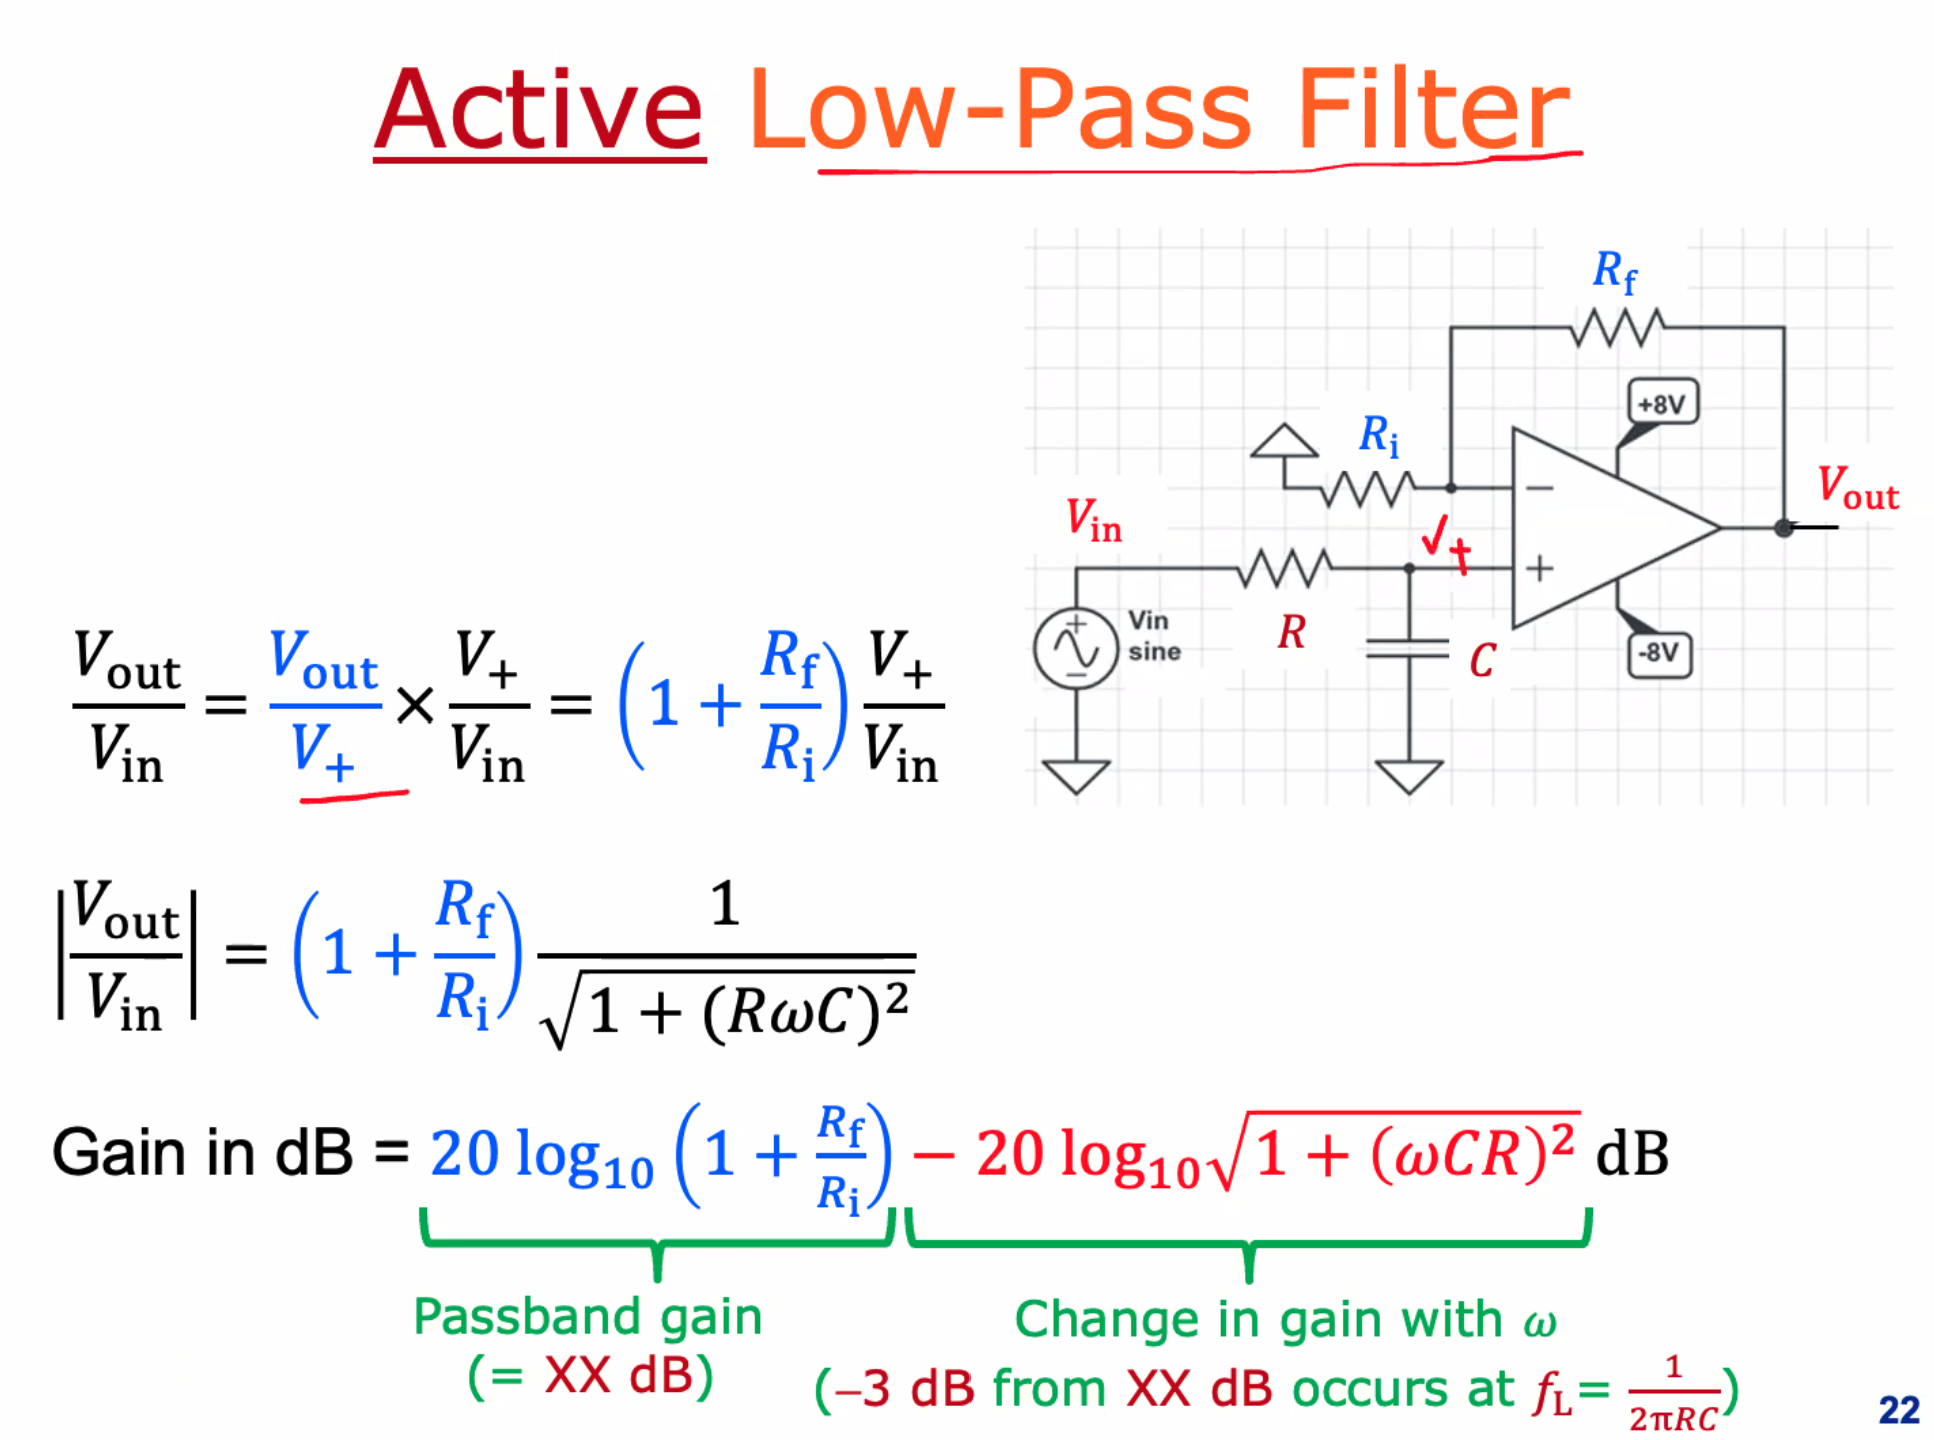
\includegraphics[width=0.9\linewidth]{images/gain-of-active-low-pass-filter.png}}
    \end{itemize}
    A point to note is that in the formula, we have $\omega$, which if not $f$, so we need to use $\omega=2\pi f$ to convert $f$ to $\omega$ and then do our calculation.
    \item (\textbf{Graph of Gain in dB vs frequency})
    \begin{itemize}
        \item (\textbf{Passive Low-Pass Filter}) \\
        \centerline{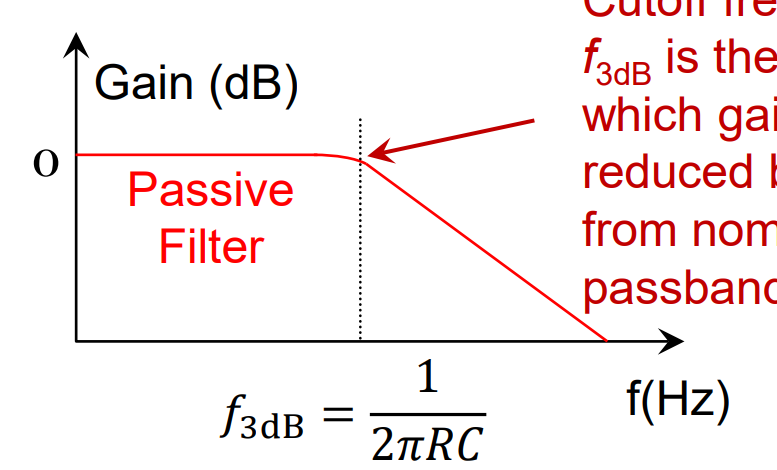
\includegraphics[width=0.5\linewidth]{images/graph-passive-low-pass-filter.png}}
        \item (\textbf{Passive High-Pass Filter}) \\
        \centerline{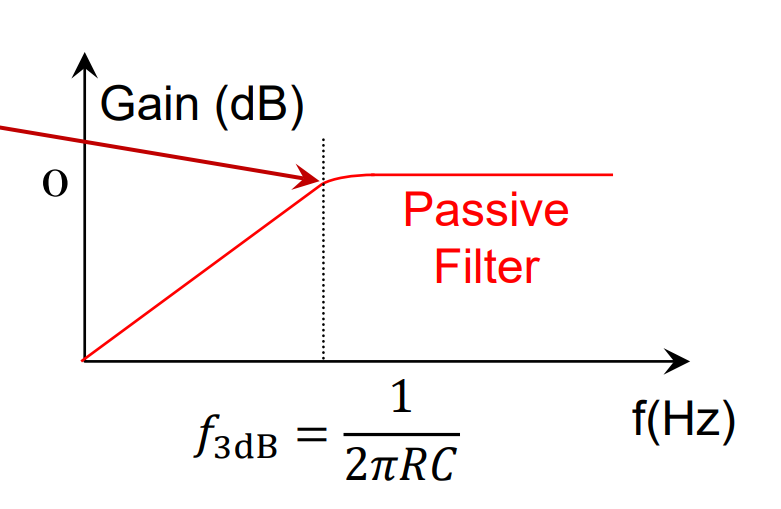
\includegraphics[width=0.5\linewidth]{images/graph-passive-high-pass-filter.png}}
    \end{itemize}
    The idea we get from these two graphs is that actually the slope will become \textbf{steeper (increase/decrease by more dB)} as we move opposite to the characteristic of the filter.
    \item (\textbf{Band Pass Filter}) It consists of a \textbf{low-pass filter} and a \textbf{high-pass filter}. The steps for solving this kind of question are:
    \begin{itemize}
        \item Divide the circuit and find the high and low pass filter.
        \item Analyze the corresponding \textbf{cut-off frequency} for the high and low pass filter respectively.
        \item Use the formula $f=\frac{1}{2\pi RC}$ to solve for $R$ and $C$.
    \end{itemize}
    To get the corresponding \textbf{cut-off frequency}, we can refer to the graph of $dB$ over $f$ below, where $f_H$ is the cut-off frequency of the high-pass filter and $f_L$ is a cut-off frequency of the low-pass filter.  \\
    \centerline{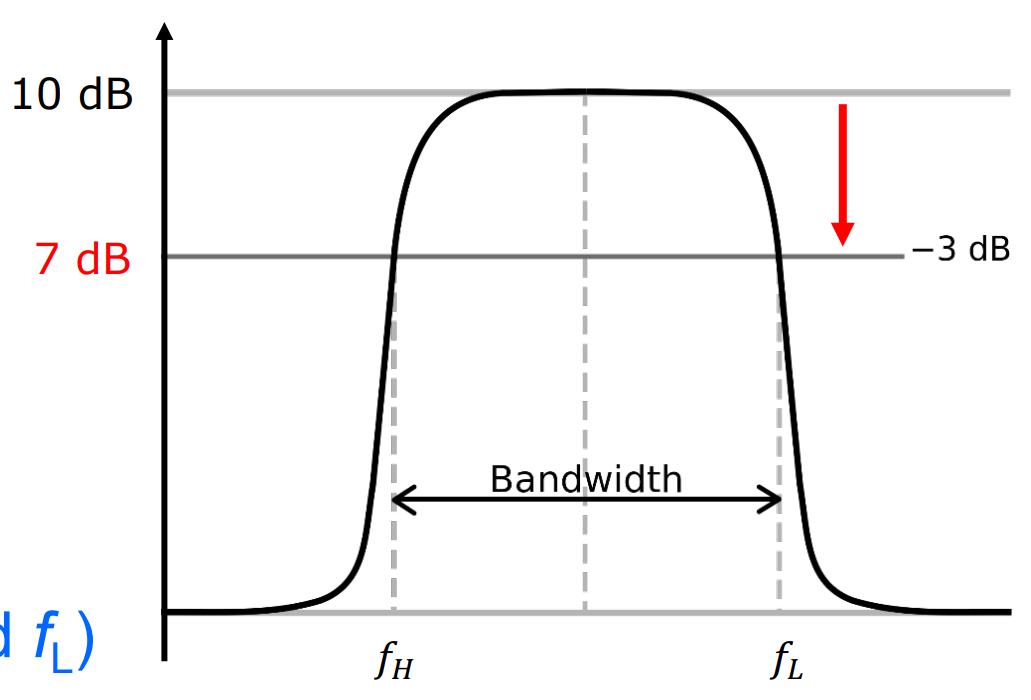
\includegraphics[width=0.5\linewidth]{images/band-pass-filter-graph.png}}
    And a band-pass filter consists of a low-pass filter first and then a high-pass filter looks like below \\
    \centerline{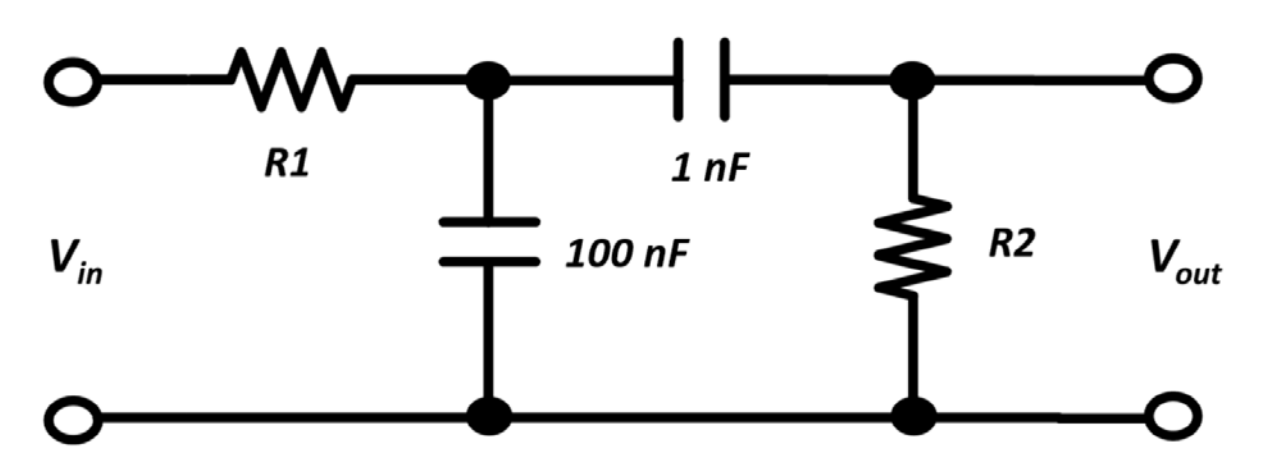
\includegraphics[width=0.7\linewidth]{images/band-pass-filter.png}}
\end{enumerate}

\section{05. (Studio 11) Acoustic Sensors}
\subsection{Ultrasonic Sensor}
\begin{enumerate}
    \item (\textbf{Working Principle}) The ultrasonic sensor head emits an ultrasonic wave, which has the speed of sound 340m/s and receives the wave reflected from the target. Then the ultrasonic will output the time between the emission and reception.
    \item (\textbf{Tips})
    \begin{itemize}
        \item The distance travelled is \textbf{2} times the distance between the target and the sensor.
    \end{itemize}
\end{enumerate}
\subsection{Microphone}
\begin{enumerate}
    \item (\textbf{Envelope Detector}) An envelop detector is an electronic circuit that takes a high-frequency signal as input (\textbf{sound}) and provides an output which is the envelope of the original signal.
    \item (\textbf{Working Principle})
    \begin{itemize}
        \item First, the input signal passes through a forward-biased diode, which will only let the \textbf{positive signal} to pass
        \item Second, it utilizes the \textbf{charging and discharging} characteristic of a capacitor. So, basically the capacitor stores up charge on the rising edge, and releases it slowly through the resistor when the signal falls.
    \end{itemize}
    \item (\textbf{Sensitivity}) The envelop detector is more accurate when $RC$ is very \textbf{small}. That's because when $RC$ is small, which is the same as $\tau$ is very small ($\tau = RC$). So, charging and discharging of the capacitor will be very \textbf{fast}. And this will make our output mostly follow our input signal. \\
    \centerline{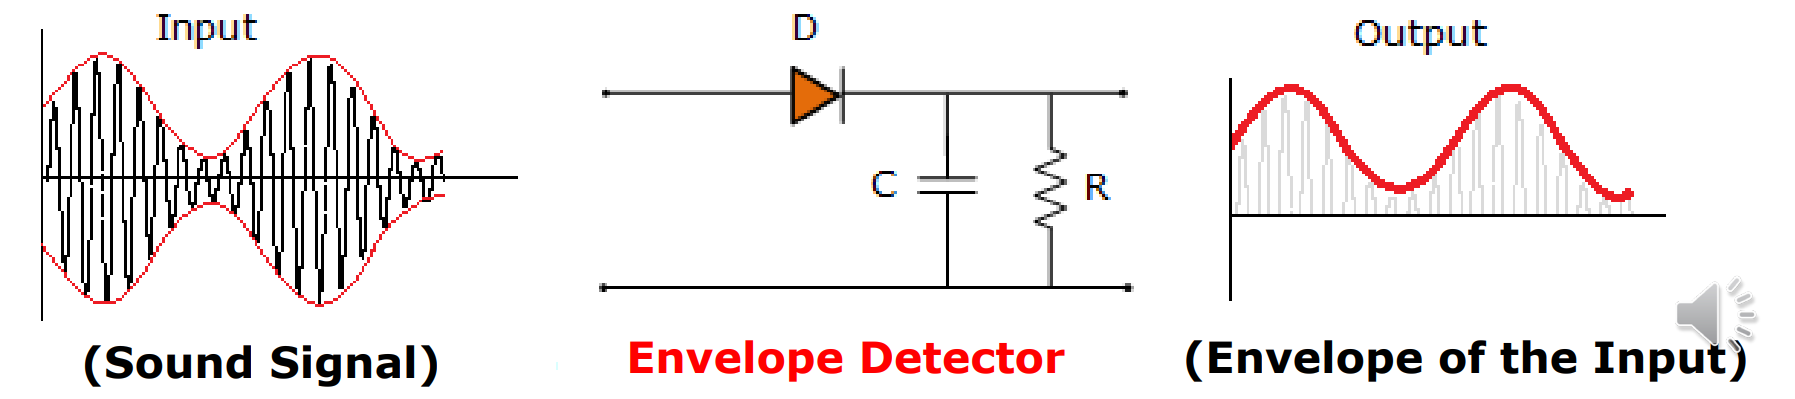
\includegraphics[width=1.0\linewidth]{images/envelop-detector.png}}
\end{enumerate}

\section{06. (Studio 12) Photoelectric Sensors}
\subsection{InfraRed Emitter \& Detector}
\begin{enumerate}
    \item (\textbf{Symbol})
    \begin{itemize}
        \item (Emitter) A special purpose LED that emits light in the InfraRed range of wavelength between 700 nm and 1 mm. \\
        \centerline{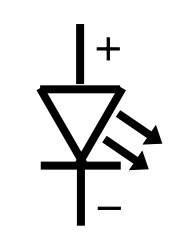
\includegraphics[width=0.1\linewidth]{images/ir-sensor-emitter-symbol.png}}
        \item (Detector) The voltage across collector (C) and emitter (E) terminals varies proportionally to the IR light received. \\
        \centerline{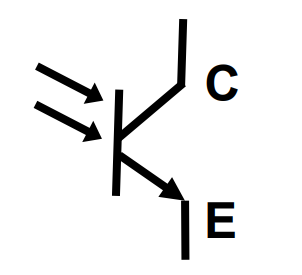
\includegraphics[width=0.1\linewidth]{images/ir-sensor-detector-symbol.png}}
    \end{itemize}
    \item (\textbf{IR Sensor}) It just combines the IR phototransistor (detector) with IR Emitter.
    \item (\textbf{Two types of Incidence})
    \begin{itemize}
        \item (IR Direct Incidence) IR Emitter is placed directly in front of the IR Detector. \\
        \centerline{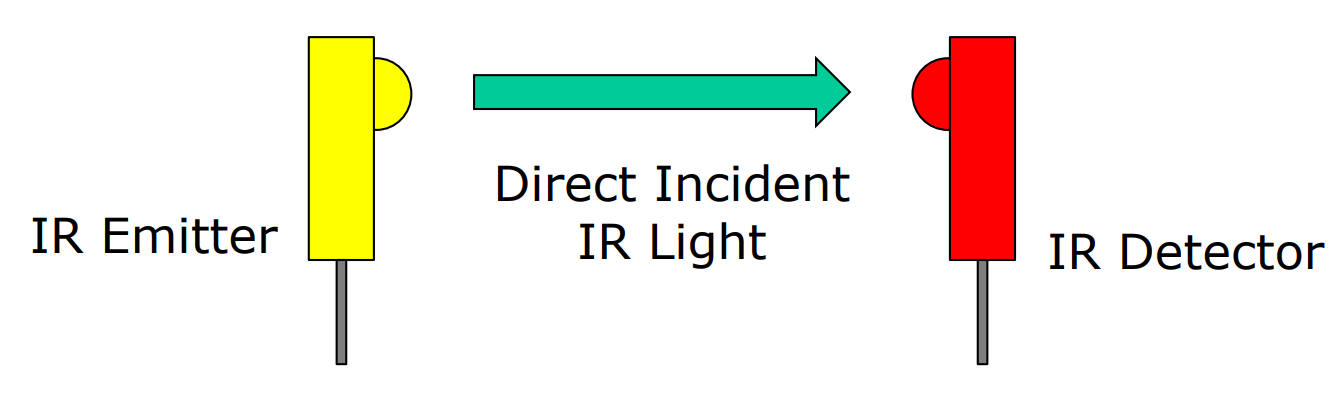
\includegraphics[width=0.5\linewidth]{images/ir-direct-incidence.png}}
        \item (IR Indirect Incidence) The IR Emitter and Detector are placed side by side with the opaque object in front of them. \\
        \centerline{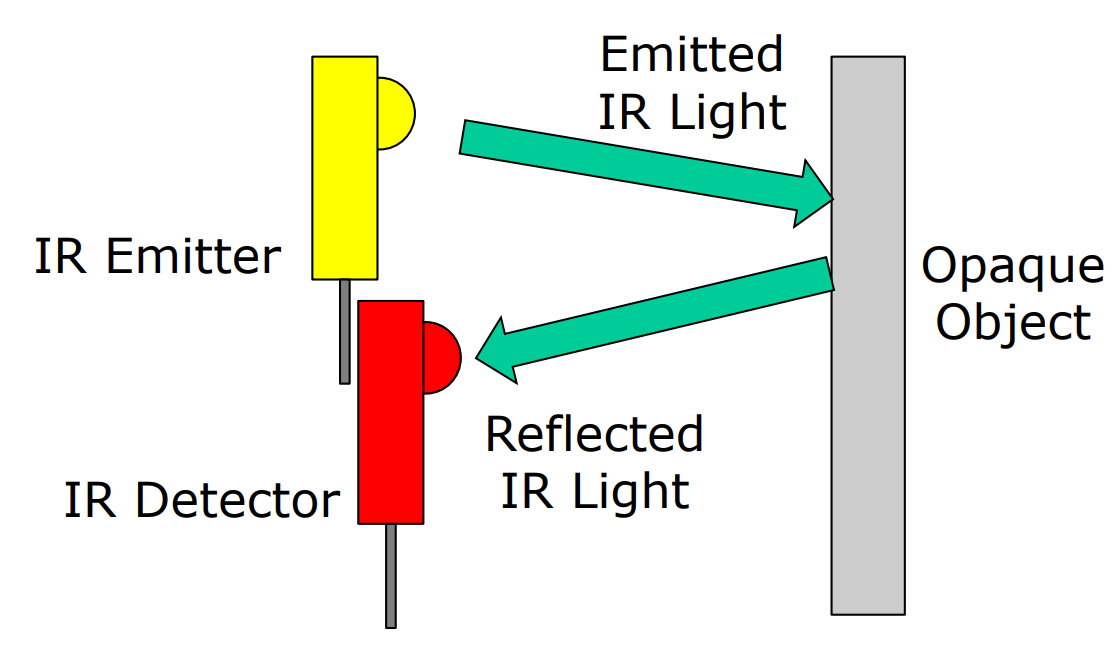
\includegraphics[width=0.4\linewidth]{images/ir-indirect-incidence.png}}
    \end{itemize}
    \item (\textbf{Optimal working range for IR sensor}) Given a graph below, the optimal working range should be 2-8 cm. \\
    \centerline{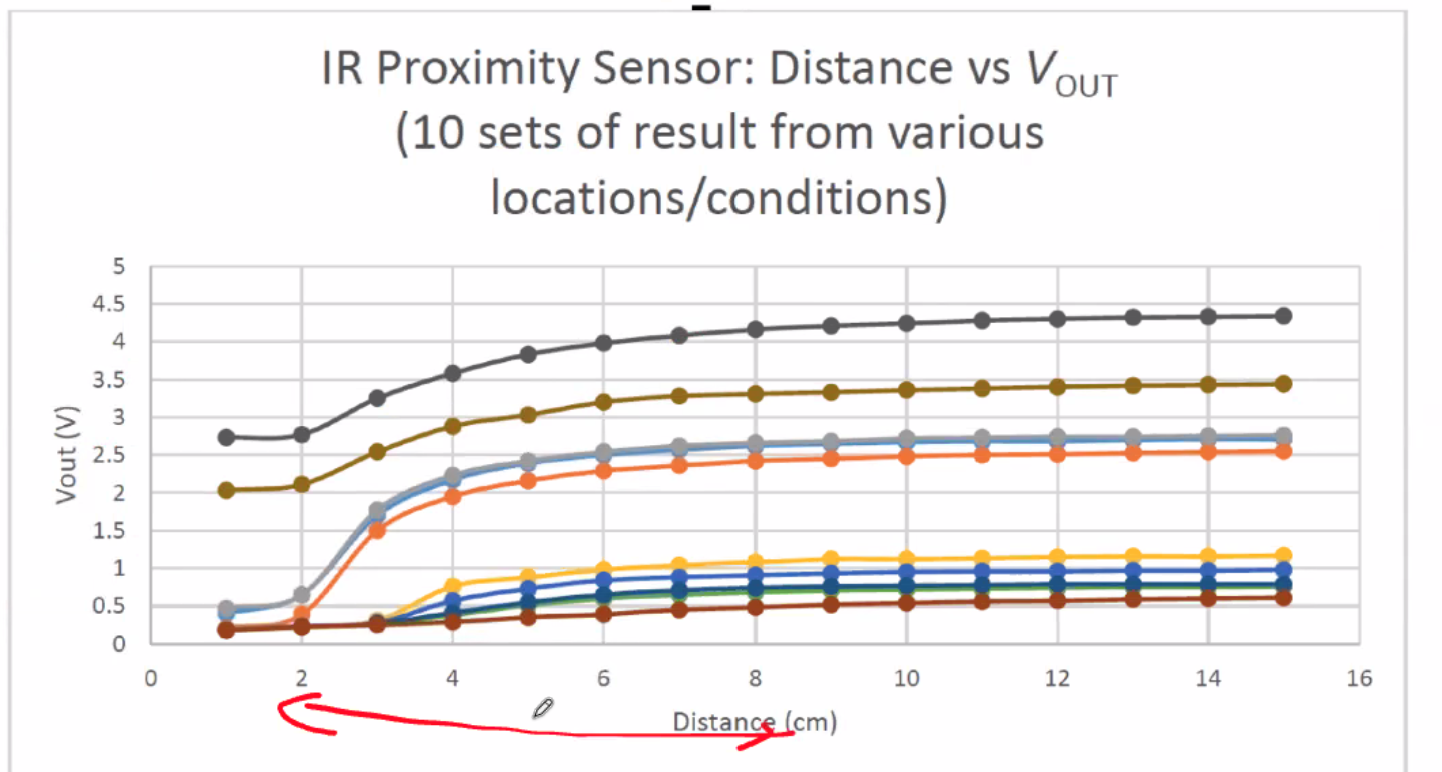
\includegraphics[width=0.9\linewidth]{images/ir-sensor-working-range.png}}
    \item (\textbf{Resistor Range}) Usually in the real-world circuit, we connect the IR sensor in series with a resistor for safety. And the range of resistance of this resistor should be \textbf{in the unit of or around $10k\Omega$}. \\
    \centerline{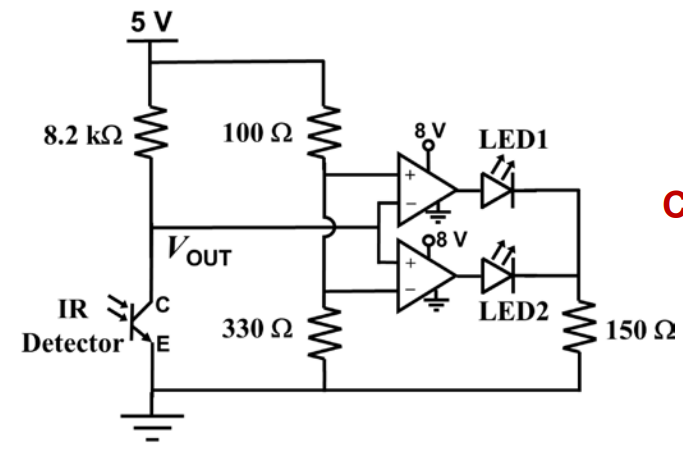
\includegraphics[width=0.9\linewidth]{images/ir-sensor-circuit.png}}
\end{enumerate}

\subsection{Light Depedent Resistor (LDR)}
\begin{enumerate}
    \item (\textbf{Main Characteristics})
    \begin{itemize}
        \item LDR is also known as Photoresistor and it is a light-controlled variable resistor
        \item The resistance of LDR varies with changes in the amount of light. \textbf{The lower the brightness, the higher its resistance}. Its illuminance vs resistance relationship is not linear! \\
        \centerline{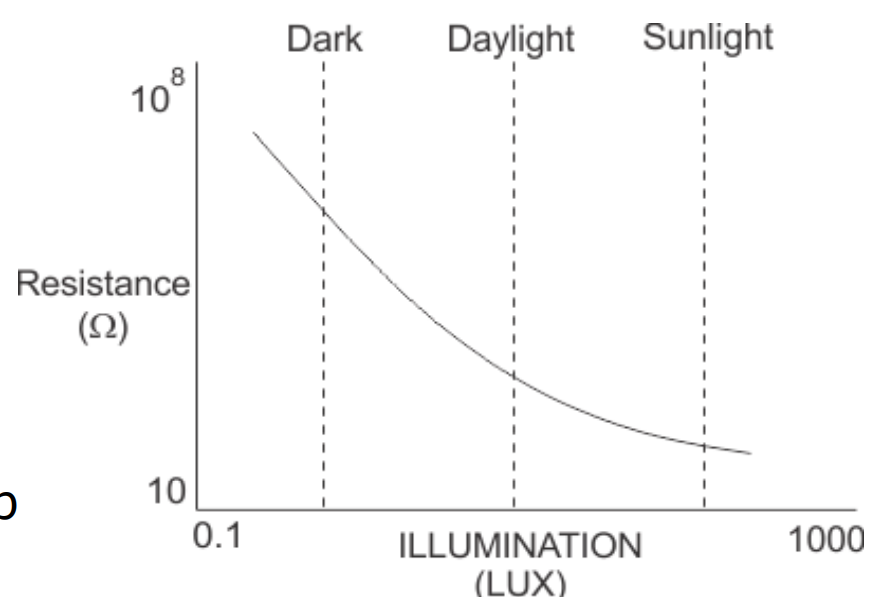
\includegraphics[width=0.7\linewidth]{images/ldr-illuminance-resistance.png}}
    \end{itemize}
    \item (\textbf{Resistor Range}) Usually in the real-world circuit, we will connect the LDR in series with a resistor for safety. And the range of the resistance of the resistor should be \textbf{in the unit of or around $100k\Omega$} \\
    For example, in the circuit below, $R_1$ can be $120k\Omega$ but it cannot be $3.3\text{M}\Omega$ since it is too big. \\
    \centerline{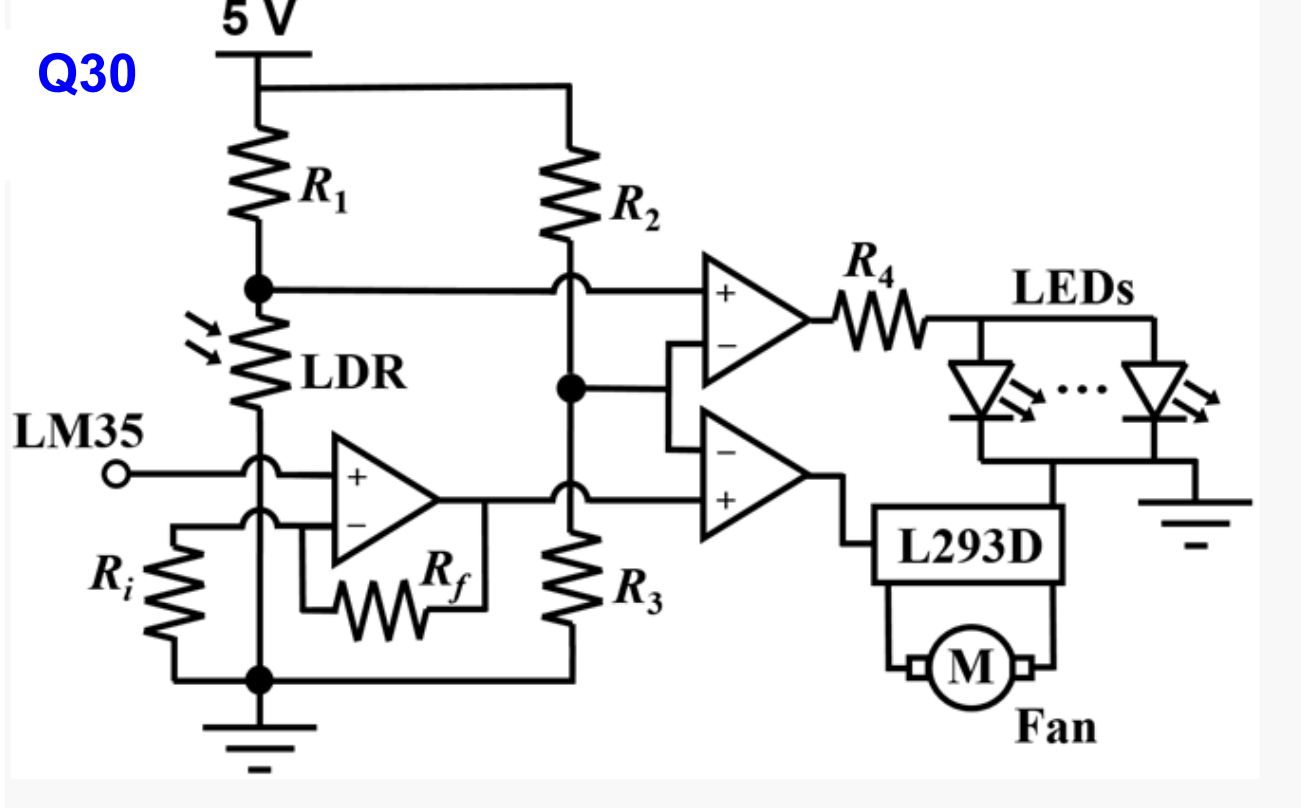
\includegraphics[width=0.8\linewidth]{images/ldr-resistor-range.png}}
\end{enumerate}
\end{multicols}

% Dividing Line
\hrulefill \\

% Tips and Notes
\begin{multicols}{3}
% Some Tips from first half
\begin{enumerate}
    \item (\textbf{RMS}) Given that an AC voltage is $v(t)=V_mcos(\omega t+\theta)=V_m\angle \theta^{\circ}$, we have $V_{\text{rms}}=\frac{V_m}{\sqrt{2}}$.
    \item (\textbf{Impedance})
    \begin{itemize}
        \item (Impedance of inductor) It is $j\omega L$. It is on the positive y-axis in phasor diagram.
        \item (Impedance of capacitor) It is $\frac{1}{j\omega C}=\frac{-j}{\omega C}$. It is on the negative y-axis in phasor diagram.
        \item (Impedance of resistor) It is $R$. It is on the positive x-axis in phasor diagram.
    \end{itemize}
    \item (\textbf{KCL on op-amp amplifier}) Please be slow and \textbf{draw the imaginary direction} of the current when using KCL!
    \item (\textbf{Graph})
    \begin{itemize}
        \item (PMDC Motor: \textbf{Fixed load}) The equation we should use is $\omega = \frac{V_m}{K_e}-\frac{R_mI_m}{K_e}$. The gradient is just $1/K_e$. Then the y-intercept helps us get the value of $R_m$.
        \item (PMDC Motor: \textbf{Fixed voltage}) The equation we should use is $I_m=\frac{V_m}{R_m}-\frac{K_e\omega}{R_m}$. Using the y-intercept ($V_m/R_m$) can easily calculate $R_m$. Then the gradient ($-\frac{K_e}{R_m}$) helps us get the value of $K_e$.
        \item (Ultrasonic sensor) The gradient of the graph about distance(cm) vs duration($\mu$s) gives the speed of the sound. Note that the unit here is cm/$\mu$s initially.
    \end{itemize}
\end{enumerate}

%QnA
%\begin{enumerate}

%    \item For other motors, do we need to know the working principles of them? Like Gear Motor?
%    \item No-load current in 0 in our test if we ignore the friction?
%    \item How the diode bridge bridge rectifier changes the ac current to dc current? And what's the use of voltage ripple?
%    \item Do we need to know the working principle of DC motors? Will it be tested in the quiz? Including why we need the commutation?
%    \item For motor efficiency, in calculation, we just treat $P_{\text{out}}$ as $P_{\text{mech}}$ and $P_{\text{in}}$ as $P_{\text{elec}}$
%    \item Do we need to know how to read the Op-amp Data sheet? And do we need to memorize the typical op-amp parameters?
%    \item Will spectral analysis be tested in quiz 2?
%    \item The application of inverting and non-inverting comparator. And its affect on the saturation voltage.
%\end{enumerate}
\end{multicols}

\end{document}
